\documentclass{article}

%%%%%%%%%%%%%%%CUSTOM ADD PACKAGES%%%%%%%%%%%
% if you need to pass options to natbib, use, e.g.:
%     \PassOptionsToPackage{numbers, compress}{natbib}
% before loading neurips_2021

% ready for submission
% \usepackage{neurips_2021}

% to compile a preprint version, e.g., for submission to arXiv, add add the
% [preprint] option:
%     \usepackage[preprint]{neurips_2021}

% to compile a camera-ready version, add the [final] option, e.g.:
\usepackage[final, nonatbib]{neurips_2021}

% to avoid loading the natbib package, add option nonatbib:
%    \usepackage[nonatbib]{neurips_2021}

\usepackage[utf8]{inputenc} % allow utf-8 input
\usepackage[T1]{fontenc}    % use 8-bit T1 fonts
\usepackage{hyperref}       % hyperlinks
\usepackage{url}            % simple URL typesetting
\usepackage{booktabs}       % professional-quality tables
\usepackage{amsfonts}       % blackboard math symbols
\usepackage{amsmath}
\usepackage{mathtools}
\usepackage{amsthm}
\usepackage{nicefrac}       % compact symbols for 1/2, etc.
\usepackage{microtype}      % microtypography
\usepackage{xcolor}         % colors
%%%%%%%%%%%%%%%CUSTOM ADD PACKAGES%%%%%%%%%%%
\usepackage{comment}
\usepackage{enumitem}
\usepackage{graphicx} 
\usepackage{lscape}
\usepackage{tcolorbox}
%\usepackage{enumerate}
% \usepackage[dvipsnames]{xcolor}
\graphicspath{Figures/}
\def\BibTeX{{\rm B\kern-.05em{\sc i\kern-.025em b}\kern-.08em
		T\kern-.1667em\lower.7ex\hbox{E}\kern-.125emX}}


%%%%%%%%%%%%%%%%%%%%%%%%%%%%%%%%%%%%%%%%%%%%%


\title{Quantum-to-Classical Randomness Extractors}

% The \author macro works with any number of authors. There are two commands
% used to separate the names and addresses of multiple authors: \And and \AND.
%
% Using \And between authors leaves it to LaTeX to determine where to break the
% lines. Using \AND forces a line break at that point. So, if LaTeX puts 3 of 4
% authors names on the first line, and the last on the second line, try using
% \AND instead of \And before the third author name.

\author{%
  Kyle Marie Astroth 
  \thanks{
    %EECS Department, University of Michigan, Ann Arbor, MI 48105 \\
    \texttt{\{kastroth,mdaamir,nehark,sriasat,jiangwf\}@umich.edu}
  } 
  \And
  Mohammad Aamir Sohail 
  \footnotemark[1]
  \And
  Neha Rama Kumar 
  \footnotemark[1]
  \And
  Samin Riasat 
  \footnotemark[1]
  \And
  Wenfan Jiang 
  \footnotemark[1]
  %\thanks{Use footnote for providing further information about author (webpage, alternative address)---\emph{not} for acknowledging funding agencies.} \\
%   EECS Department\\
%   University of Michigan\\
%   Ann Arbor, MI 48105 \\
%   \texttt{knouman@umich.edu} \\
%   % examples of more authors
%   \And
%   Unique Name: mdaamir, UMID: 13292672\\
%   University of Michigan\\
%   Ann Arbor, MI 48105 \\
%   \texttt{mdaamir@umich.edu}
%   \AND
  % Address \\
  % \texttt{email} \\
    % \And
  % Coauthor \\
  % Affiliation \\
  % Address \\
  % \texttt{email} \\
    % \And
  % Coauthor \\
  % Affiliation \\
  % Address \\
  % \texttt{email} \\
}
%=======================================
%%% BLACKBOARD SYMBOLS

\newcommand{\C}{\ensuremath{\mathbb{C}}}
\newcommand{\D}{\ensuremath{\mathbb{D}}}
\newcommand{\E}{\ensuremath{\mathbb{E}}}
\newcommand{\I}{\ensuremath{\mathbb{I}}}
\newcommand{\G}{\ensuremath{\mathbb{G}}}
\newcommand{\J}{\ensuremath{\mathbb{J}}}
\newcommand{\N}{\ensuremath{\mathbb{N}}}
\newcommand{\Q}{\ensuremath{\mathbb{Q}}}
\newcommand{\R}{\ensuremath{\mathbb{R}}}
\newcommand{\T}{\ensuremath{\mathbb{T}}}
\newcommand{\Z}{\ensuremath{\mathbb{Z}}}
\newcommand{\QR}{\ensuremath{\mathbb{QR}}}

\newcommand{\Zt}{\ensuremath{\Z_t}}
\newcommand{\Zp}{\ensuremath{\Z_p}}
\newcommand{\Zq}{\ensuremath{\Z_q}}
\newcommand{\ZN}{\ensuremath{\Z_N}}
\newcommand{\Zps}{\ensuremath{\Z_p^*}}
\newcommand{\ZNs}{\ensuremath{\Z_N^*}}
\newcommand{\JN}{\ensuremath{\J_N}}
\newcommand{\QRN}{\ensuremath{\QR_{N}}}
\newcommand{\QRp}{\ensuremath{\QR_{p}}}

%%% THEOREM COMMANDS

\theoremstyle{plain}            % following are "theorem" style
\newtheorem{theorem}{Theorem}[section]
\newtheorem{lemma}[theorem]{Lemma}
\newtheorem{corollary}[theorem]{Corollary}
\newtheorem{proposition}[theorem]{Proposition}
% \newtheorem{claim}[theorem]{Claim}
\newtheorem{fact}[theorem]{Fact}

\theoremstyle{definition}       % following are def style
\newtheorem{definition}[theorem]{Definition}
\newtheorem{conjecture}[theorem]{Conjecture}
\newtheorem{example}[theorem]{Example}
\newtheorem{protocol}[theorem]{Protocol}

\theoremstyle{remark}           % following are remark style
\newtheorem{remark}[theorem]{Remark}
\newtheorem{note}[theorem]{Note}
% \newtheorem{exercise}[theorem]{Exercise}

% equation numbering style
\numberwithin{equation}{section}

% section reference style
\renewcommand{\sectionautorefname}{\S}

%%% GENERAL COMPUTING

\newcommand{\bit}{\ensuremath{\set{0,1}}}
\newcommand{\pmone}{\ensuremath{\set{-1,1}}}
\newcommand{\eps}{\ensuremath{\varepsilon}}
\newcommand{\bra}[1]{\langle #1|}
\newcommand{\ket}[1]{|#1 \rangle}
\newcommand{\braket}[2]{\langle #1 | #2 \rangle}

% asymptotics
\DeclareMathOperator{\Tr}{Tr}
\DeclareMathOperator{\poly}{poly}
\DeclareMathOperator{\polylog}{polylog}
\DeclareMathOperator{\negl}{negl}
\newcommand{\Otil}{\ensuremath{\tilde{O}}}

% probability/distribution stuff
% \DeclareMathOperator*{\E}{E}
\DeclareMathOperator*{\Var}{Var}

% sets in calligraphic type
\newcommand{\calB}{\ensuremath{\mathcal{B}}}
\newcommand{\calD}{\ensuremath{\mathcal{D}}}
\newcommand{\calF}{\ensuremath{\mathcal{F}}}
\newcommand{\calG}{\ensuremath{\mathcal{G}}}
\newcommand{\calH}{\ensuremath{\mathcal{H}}}
\newcommand{\Ii}{\mathcal{I}}
\newcommand{\calL}{\ensuremath{\mathcal{L}}}
\newcommand{\calP}{\ensuremath{\mathcal{P}}}
\newcommand{\calS}{\ensuremath{\mathcal{S}}}
\newcommand{\calT}{\ensuremath{\mathcal{T}}}
\newcommand{\calX}{\ensuremath{\mathcal{X}}}
\newcommand{\calY}{\ensuremath{\mathcal{Y}}}
\newcommand{\calV}{\ensuremath{\mathcal{V}}}
\newcommand{\Hmin}{H_{{\min}}}

% types of indistinguishability
\newcommand{\compind}{\ensuremath{\stackrel{c}{\approx}}}
\newcommand{\statind}{\ensuremath{\stackrel{s}{\approx}}}
\newcommand{\perfind}{\ensuremath{\equiv}}

% font for general-purpose algorithms
\newcommand{\algo}[1]{\ensuremath{\mathsf{#1}}}
% font for general-purpose computational problems
\newcommand{\problem}[1]{\ensuremath{\mathsf{#1}}}
% font for complexity classes
\newcommand{\class}[1]{\ensuremath{\mathsf{#1}}}

% complexity classes and languages
\renewcommand{\P}{\class{P}}
\newcommand{\BPP}{\class{BPP}}
\newcommand{\NP}{\class{NP}}
\newcommand{\coNP}{\class{coNP}}
\newcommand{\AM}{\class{AM}}
\newcommand{\coAM}{\class{coAM}}
\newcommand{\IP}{\class{IP}}

%%% "LEFT-RIGHT" PAIRS OF SYMBOLS

%% NOTE: this requires \usepackage{mathtools} in the document preamble
% norm
\DeclarePairedDelimiter\norm{\|}{\|}
% inner product
\DeclarePairedDelimiter\inner{\langle}{\rangle}
% absolute value
\DeclarePairedDelimiter\abs{\lvert}{\rvert}
% a set
\DeclarePairedDelimiter\set{\{}{\}}
% parens
\DeclarePairedDelimiter\parens{(}{)}
% tuple, alias for parens
\DeclarePairedDelimiter\tuple{(}{)}
% square brackets
\DeclarePairedDelimiter\bracks{[}{]}
% rounding off
\DeclarePairedDelimiter\round{\lfloor}{\rceil}
% floor function
\DeclarePairedDelimiter\floor{\lfloor}{\rfloor}
% ceiling function
\DeclarePairedDelimiter\ceil{\lceil}{\rceil}
% length of some vector, element
\DeclarePairedDelimiter\length{\lVert}{\rVert}
% "lifting" of a residue class
\DeclarePairedDelimiter\lift{\llbracket}{\rrbracket}
\DeclarePairedDelimiter\len{\lvert}{\rvert}

%%% CRYPTO-RELATED NOTATION

% KEYS AND RELATED

\newcommand{\key}[1]{\ensuremath{#1}}

\newcommand{\pk}{\key{pk}}
\newcommand{\vk}{\key{vk}}
\newcommand{\sk}{\key{sk}}
\newcommand{\mpk}{\key{mpk}}
\newcommand{\msk}{\key{msk}}
\newcommand{\fk}{\key{fk}}
\newcommand{\id}{id}
\newcommand{\keyspace}{\ensuremath{\mathcal{K}}}
\newcommand{\msgspace}{\ensuremath{\mathcal{M}}}
\newcommand{\ctspace}{\ensuremath{\mathcal{C}}}
\newcommand{\tagspace}{\ensuremath{\mathcal{T}}}
\newcommand{\idspace}{\ensuremath{\mathcal{ID}}}

\newcommand{\concat}{\ensuremath{\|}}

% GAMES

% advantage
\newcommand{\advan}{\ensuremath{\mathbf{Adv}}}

% different attack models
\newcommand{\attack}[1]{\ensuremath{\text{#1}}}

\newcommand{\atk}{\attack{atk}} % dummy attack
\newcommand{\indcpa}{\attack{ind-cpa}}
\newcommand{\indcca}{\attack{ind-cca}}
\newcommand{\anocpa}{\attack{ano-cpa}} % anonymous
\newcommand{\anocca}{\attack{ano-cca}}
\newcommand{\euacma}{\attack{eu-acma}} % forgery: adaptive chosen-message
\newcommand{\euscma}{\attack{eu-scma}} % forgery: static chosen-message
\newcommand{\suacma}{\attack{su-acma}} % strongly unforgeable

% ADVERSARIES
\newcommand{\attacker}[1]{\ensuremath{\mathcal{#1}}}

\newcommand{\Adv}{\attacker{A}}
\newcommand{\AdvA}{\attacker{A}}
\newcommand{\AdvB}{\attacker{B}}
\newcommand{\Dist}{\attacker{D}}
\newcommand{\Sim}{\attacker{S}}
\newcommand{\Ora}{\attacker{O}}
\newcommand{\Inv}{\attacker{I}}
% \newcommand{\For}{\attacker{F}}

% CRYPTO SCHEMES

\newcommand{\scheme}[1]{\ensuremath{\text{#1}}}

% pseudorandom stuff
\newcommand{\prg}{\algo{PRG}}
\newcommand{\prf}{\algo{PRF}}
\newcommand{\prp}{\algo{PRP}}

% symmetric-key cryptosystem
\newcommand{\skc}{\scheme{SKC}}
\newcommand{\skcgen}{\algo{Gen}}
\newcommand{\skcenc}{\algo{Enc}}
\newcommand{\skcdec}{\algo{Dec}}

% public-key cryptosystem
\newcommand{\pkc}{\scheme{PKC}}
\newcommand{\pkcgen}{\algo{Gen}}
\newcommand{\pkcenc}{\algo{Enc}} % can also use \kemenc and \kemdec
\newcommand{\pkcdec}{\algo{Dec}}

% digital signatures
\newcommand{\sig}{\scheme{SIG}}
\newcommand{\siggen}{\algo{Gen}}
\newcommand{\sigsign}{\algo{Sign}}
\newcommand{\sigver}{\algo{Ver}}

% message authentication code
\newcommand{\mac}{\scheme{MAC}}
\newcommand{\macgen}{\algo{Gen}}
\newcommand{\mactag}{\algo{Tag}}
\newcommand{\macver}{\algo{Ver}}

% key-encapsulation mechanism
\newcommand{\kem}{\scheme{KEM}}
\newcommand{\kemgen}{\algo{Gen}}
\newcommand{\kemenc}{\algo{Encaps}}
\newcommand{\kemdec}{\algo{Decaps}}

% identity-based encryption
\newcommand{\ibe}{\scheme{IBE}}
\newcommand{\ibesetup}{\algo{Setup}}
\newcommand{\ibeext}{\algo{Ext}}
\newcommand{\ibeenc}{\algo{Enc}}
\newcommand{\ibedec}{\algo{Dec}}

% hierarchical IBE (as key encapsulation)
\newcommand{\hibe}{\scheme{HIBE}}
\newcommand{\hibesetup}{\algo{Setup}}
\newcommand{\hibeext}{\algo{Extract}}
\newcommand{\hibeenc}{\algo{Encaps}}
\newcommand{\hibedec}{\algo{Decaps}}

% binary tree encryption (as key encapsulation)
\newcommand{\bte}{\scheme{BTE}}
\newcommand{\btesetup}{\algo{Setup}}
\newcommand{\bteext}{\algo{Extract}}
\newcommand{\bteenc}{\algo{Encaps}}
\newcommand{\btedec}{\algo{Decaps}}

% trapdoor functions
\newcommand{\tdf}{\scheme{TDF}}
\newcommand{\tdfgen}{\algo{Gen}}
\newcommand{\tdfeval}{\algo{Eval}}
\newcommand{\tdfinv}{\algo{Invert}}
\newcommand{\tdfver}{\algo{Ver}}

%%% PROTOCOLS

\newcommand{\out}{\text{out}}
\newcommand{\view}{\text{view}}

%%% TIKZ LIBRARIES
\usepackage{tikz}
\usetikzlibrary{shapes, calc}

%%% COMMANDS FOR LECTURES/HOMEWORKS

\newcommand{\lecheader}{%
  \chead{\large \textbf{Lecture \lecturenum\\\lecturetopic}}

  \setlength{\headheight}{20pt}
  \setlength{\headsep}{16pt}
}

\newcommand{\hwheader}{%
  \chead{\Large \textbf{Homework \hwnum}}

  \setlength{\headheight}{20pt}
  \setlength{\headsep}{16pt}
  
  \headrule
}

\newcommand{\discussionheader}{%
  \chead{\Large \textbf{Discussion \discussionnum}}
  
  \rhead{\small \textbf{\discussiontopic \\ \discussiondate}}
  
  \setlength{\headheight}{20pt}
  \setlength{\headsep}{16pt}
  
  \headrule
}

\newcommand{\examheader}{%
  \chead{\Large \textbf{Take-Home Exam \examnum}}
  

  \setlength{\headheight}{20pt}
  \setlength{\headsep}{16pt}
  
  \headrule
}
  
%=======================================
\begin{document}

\maketitle

\begin{abstract}
  Randomness is an essential resource for information theory, cryptography, and computation. The goal of randomness extraction is to distill (almost) perfect randomness from a weak source of randomness. In this report, we first define classical randomness extractors, or when the source of randomness yields a classical string $X$. When considering a physical randomness source, $X$ is itself ultimately the result of a measurement on an underlying quantum system, and the question arises of how much classical randomness can we extract from a quantum system. To understand and analyze this question, we will first provide the relevant quantum preliminary background, and then define quantum-to-classical (QC) and quantum-to-quantum (QQ) randomness extractors. Finally, we will explore cryptographic applications of QC randomness extractors, such as security in the noisy-storage model, and discuss possible future applications, such as privacy amplification.
\end{abstract}
%%% [Final report] Abstract should convey that we started from classical and then "When considering a physical randomness source, X is itself ultimately the result of a measurement on an underlying quantum system, and the question arises of how much classical randomness can we extract from a quantum system"... then we discuss QC, also touched upon QQ and finally applications.

\tableofcontents

%%% Includes brief description about each of the chapter.
\section{Introduction}\label{sec:intro}
Randomized algorithms are algorithms that use a degree of randomness as part of their logic. Randomized algorithms frequently outperform and simplify the best-known deterministic algorithms, and sources of randomness are a powerful but evasive resource. Further, access to randomness is an essential tool for cryptography. Randomized algorithms are designed and studied under the assumption that computers have access to true randomness in the form of a sequence of truly random bits. However, this randomness is taken from sources that only appear to have randomness, otherwise known as entropy. Entropy is a term borrowed from physics that refers to the amount of "disorder" in a system and is the measure of the uncertainty associated with a random variable. Some examples of these sources of randomness are generating and measuring electromagnetic or radioactive noise, measuring the timing of past events, or measuring user-dependent behavior \cite{Shaltiel2011}. The goal of randomness extraction is to convert these weak sources of randomness into uniformly random bits, which are measured in terms of the min-entropy. A visual representation of this process can be seen in \autoref{fig:HighlevelDiagram}. This has led to the research and development of Classical Randomness Extractors (CC-Extractors). In Section 2, we give a thorough introduce the two main concepts of Classical Randomness Extractors, deterministic and seeded extractors. %%% [Final Report] We000 briefly discuss about few construction of CC extractor. 

\begin{figure}[!htb]
    \centering
    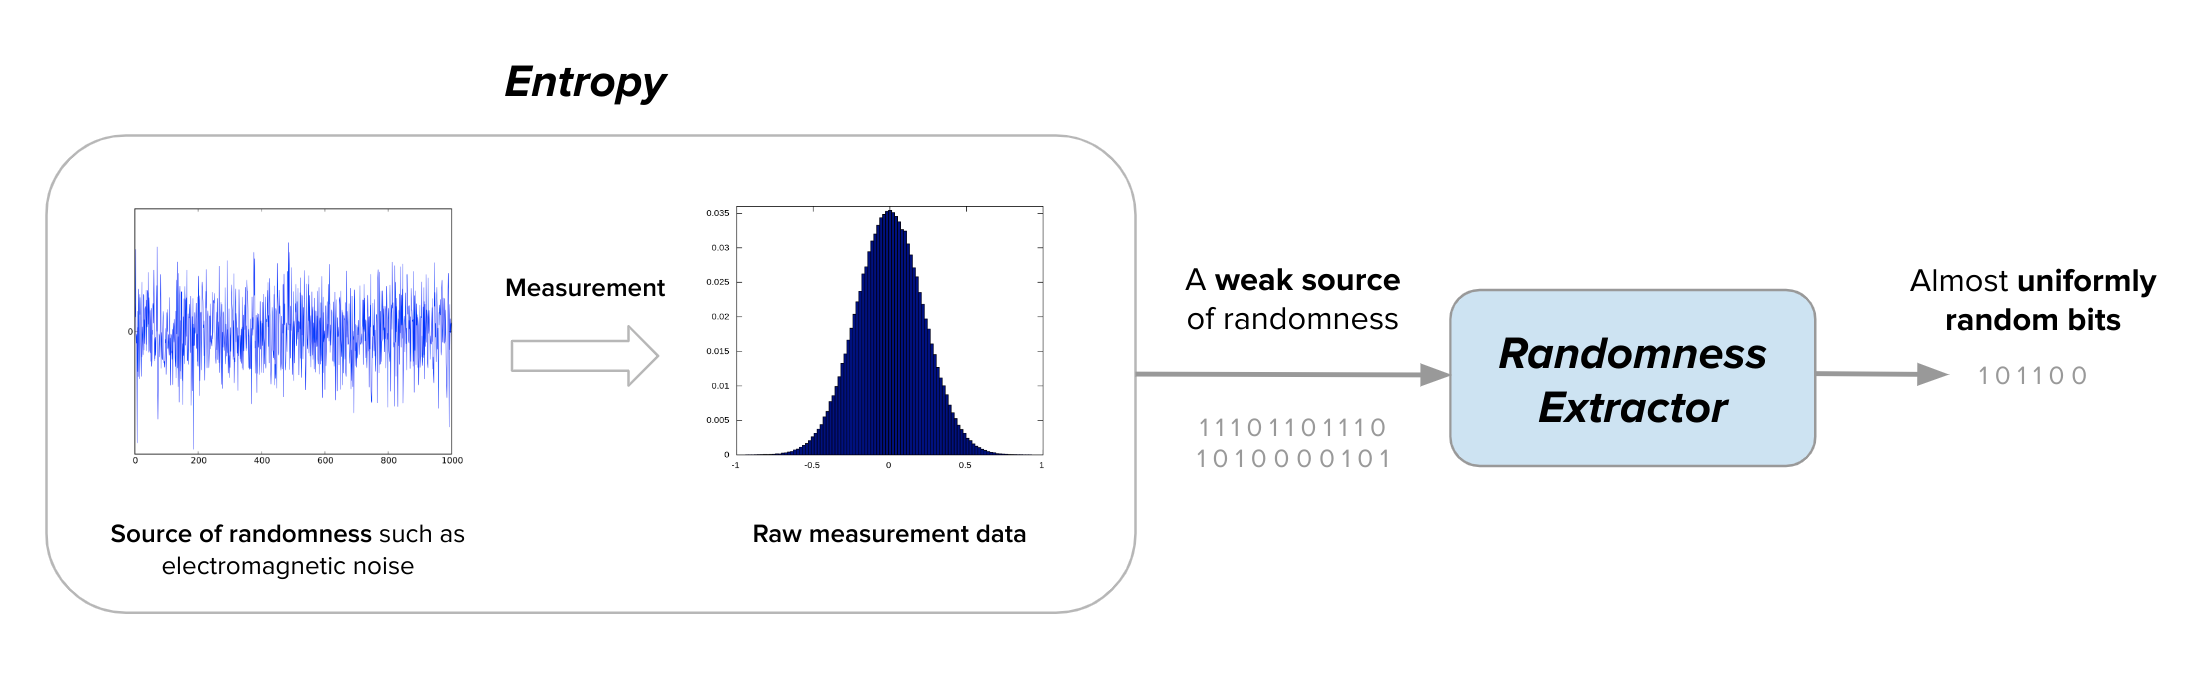
\includegraphics[scale=0.18]{Images/Highlevel_extractor.png}
    \caption{High-level diagram of a randomness extractor}
    \label{fig:HighlevelDiagram}
\end{figure}

We now know, however, that the underlying world is not classical but rather quantum, resulting in the development of quantum mechanics. %% add references
Subsequently, a randomness extractor may hold quantum side information about its (almost) uniformly random output sequence, $X$. This realization lends to several questions: where do $X$ come from? How can we hope to harness even weak sources to obtain a surplus of classical randomness? How much randomness can we obtain from a quantum source rather than a classical string? \cite{Berta_2014} Questions such as these have culminated in the study of Quantum-to-Classical Randomness Extractors (QC-Extractors) with the goal of determining how we can extract classical randomness from a physical source by performing measurements on the quantum state of said source. In contrast to the classical world, quantum mechanics allow for the creation of true randomness given the correct circumstances. It is also important to note that in a quantum setting, there also exist Quantum-to-Quantum Randomness Extractors (QQ-Extractors) that we do not measure but determine if the resulting state is quantumly fully random (maximally mixed) and uncorrelated from the extractor. In Section 3, we introduce the necessary background quantum preliminaries, and in Section 4, we discuss the construction and evaluation of QC and QQ Randomness Extractors.

Finally, we will conclude our report in Section 5 by examining the applications of QC-Extractors to entropic uncertainty relations and cryptographic problems such as noisy storage models, and Section 6 where we explore future directions of this work. Entropic uncertainty relations are fundamental to quantum mechanics and crucial tools for quantum cryptography. We will provide and discuss the proof from \cite{Berta_2014} that any set of measurements forming a QC-extractor yields an entropic uncertainty relation with respect to quantum side information and thereby obtain relations both for the Shannon and the min-entropy. The second application we will discuss is proving security in the noisy-storage model. The noisy-storage model is a quantum cryptographic model that assumes an adversary is imperfect or noisy. The study of QC extractors can further be extended to other cryptographic problems, for example, privacy amplification. We refer the curious reader to the following articles, lecture notes, and textbooks \cite{Berta_2014,tudelftQC,lo2007quantum,bruss2007quantum, bernstein2009introduction,bennett1992quantum,berta2013quantum,wilde2013quantum,nielsen2002quantum} for further reading on quantum cryptography.    

\section{Classical Randomness Extractors}\label{sec:c_ext}
As discussed in \autoref{sec:intro}, randomness extraction is an efficient procedure for taking a sample from an imperfect random source, $X$ with distribution $p_X$, and "extracting" the \textit{pure}-randomness, i.e. being closer to uniformly distributed. A randomness extractor is a function that is applied to the output of a weakly random entropy source along with a short, uniformly random seed as input, and generates a highly random output that appears close to uniformly distributed and independent from the source \cite{vadhan2012}. Before formally defining a randomness extractor, we will define entropy, or how we measure the amount of randomness contained in a weak random source, as well as the statistical distance, or how we measure the closeness of the output distribution to the uniform distribution.

\begin{definition}\normalfont{\textbf{(Entropy)}}\label{def:entropy}
    The Shannon Entropy of a discrete random variable $X$ is defined as\[
        H(X) = \E\left[\log \frac{1}{p_i}\right] = \sum_{i \in X}p_i \log \frac{1}{p_i},
    \] where $p_i = \Pr[X=i]$.
\end{definition}

\begin{definition}\normalfont{\textbf{(Min- Entropy)}}\label{def:min_entropy}
    The min-entropy of a discrete random variable X is
    \[
        H_{\min}(X) = \min_{i} \log \frac{1}{p_i},
    \] or $H_{\min}(X)$ is the largest value of $k$ such that all outcomes have the probability of at most $2^{-k}$. 
    
In general, we like to guess the most likely outcome, and the probability that we are correct is $P_{\text{guess}}(X) = \max_x p_X(x)$. This results in an operational interpretation of the min-entropy as 
    \[
        H_{\min}(X) = -\log P_{\text{guess}}(X).
    \]
\end{definition}

When considering the above definitions, the question arises of why we use the min-entropy as the measure of uncertainty in cryptography as opposed to the Shannon entropy, which is used in information theory. Following Shannon’s approach, $i(x) =  -\log p_X(x)$ is the information gained when we observe $X$. Thus the Shannon entropy measured the average information gained, i.e.,  $H(X) = \sum_x p_X(x) i(x)$. However, when studying cryptography, we are interested in the worst case, not the average case, and the min-entropy $H_{\min}(X) = \min _x i(x)$ is precisely the smallest information gained. \autoref{fig:min_entropy} shows the difference between these quantities for a binary random variable. In general, $0\leq H_{\min}(X) \leq H(X)$.
\begin{figure}[!htb]
    \centering
    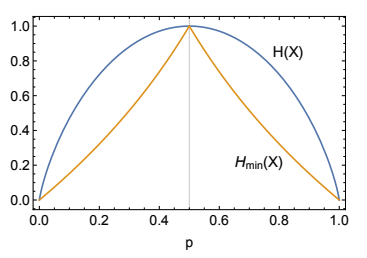
\includegraphics[scale=0.6]{Images/entropy.png}
    \caption{The comparison between Shannon entropy $H(X)$ and $\min$-entropy $H_{\min}(X)$ for a binary random variable $X = \set{0,1}$.}
    \label{fig:min_entropy}
\end{figure}

\begin{definition}\normalfont{\textbf{(Conditional Min-Entropy)}}
Consider two dependent random variables $X$ and $E$. The conditional min-entropy $H_{\min}(X|E)$ can be written as
\[H_{\min}(X|E) = -\log P_{\text{guess}}(X|E),\]
where $P_{\text{guess}}(X|E) = \max_x p_{X|E}(x|E)$.
\end{definition}

\begin{definition}\normalfont{\textbf{(Statistical Distance)}}
    Let $X$ and $Y$ be two random variables with range $\Ii$. Then the statistical distance between $X$ and $Y$ is defined as
    \[
        \Delta(X, Y) \equiv \frac{1}{2} \sum_{i \in \Ii} \left|\Pr[X=i]-\Pr[Y=i]\right|.
    \]
    For $\varepsilon \geq 0$, we define the notion of two distributions being $\varepsilon$-close as
    \[
        X \approx_{\varepsilon} Y \iff \Delta(X, Y) \leq \varepsilon.
    \]
\end{definition}

We now formally illustrate the process of randomness extraction. Consider a single party, Alice, who has access to an $n$-bit string, $x^n$, obtained from a source $X$ with distribution $p_{X}$. Perhaps, source $X$ is correlated to an additional
system or environment $E$. For example, $E$ could contain information about the generation of the source $X$ or an adversary who has gathered some prior information from protocols that include $X$. Alice has no access to system $E$ except the lower bound on the min-entropy of the source $X$ given environment $E$, i.e., $H_{\min}(X|E) \geq k$. In the task of randomness extraction, Alice’s goal is to construct \textit{randomness extractor}, denoted as $\ibeext$, that produces a
$m$-bit string $z^m$, which is close to the uniform distribution in the statistical distance and uncorrelated with environment $E$.

Before formally discussing the construction of a randomness extractor, consider an example that shows how to extract uniform bits from an i.i.d. (\textit{independent and identically distributed}) source.

\begin{example}Consider an i.i.d. binary source $X$ such that $X_i = 0$ w.p $p_0 = 1/4$ and $X_i = 1$ w.p $p_0 = 3/4$. Define the output $Z$ of the randomness extractor $Z = \ibeext(X) := X_1\oplus X_2\oplus \cdots \oplus X_n \in \set{0,1}$, i.e., the parity of all $n$-bits sequence of $X$. To find if we can extract uniformly random bits from an i.i.d. source, we need to show that $\Pr(Z=0) \approx 1/2 \pm \varepsilon$ for sufficiently small $\varepsilon > 0$, i.e., $Z \approx_{\varepsilon} \text{uniform}(\set{0,1})$.

Let's first examine how efficiently our strategy works for $n=2$. We need to compute
    $\Pr(Z=0) = \Pr(X_1 = 0, X_2 = 0) + \Pr(X_1 = 1, X_2 = 1) = p_0^2+p_1^2 = 0.625$. Similarly, we can compute $\Pr(Z=1) = 0.375$. Also, observe that $\Delta(X,U_2) = 0.25$ and $\Delta(Z,U_2) = 0.125$, where $U_2 \sim \text{uniform}(\set{0,1})$. In other words, the output distribution is not quite uniform, however, $Z$ is more closer to uniform distribution than $X$. Hence, following the above analysis for sufficiently large $n$, we observe that $Z \approx_\varepsilon U_2$.

\end{example}

In the above example, we considered a function that takes only the source $X$ as input. We call such functions deterministic or seedless extractors. Ideally, we wish to construct a deterministic extractor that, given a source of randomness with high min-entropy, outputs a distribution that is statistically close to random and near-perfect randomness without requiring an additional source of randomness.  However, in reality, there does not exist a fixed deterministic
procedure that can be used to extract even a single bit of randomness from a source with $H_{\min}(X) \geq k$,
even when $k = n - 1$. The following proposition provides the proof that it is not possible to construct a deterministic extractor.

\begin{proposition}
    Let $\ibeext:\{0,1\}^n \rightarrow \{0,1\}^m$ be a function taking input from a source. There exists a weak random source $X$ with $H_{\min} = n-1$ such that for $m=1$, $\ibeext(X)$ is a constant function.
\end{proposition}
\begin{proof}
    As defined above, $\ibeext$ outputs a single bit and must output either 0 or 1 with probability $\geq \frac{1}{2}$. Suppose $\ibeext$ outputs $0$, and define $X$ to be the flat distribution on $S = \{x : \ibeext(x) = 0\}$. Then $X$ has min-entropy of at least $n-1$, but $\Pr[\ibeext(X) = 0] = 1$, meaning the output distribution of $\ibeext$ must be a constant.
\end{proof}

Therefore, in order to construct a randomness extractor, we must also provide additional input, a seed, that is uniformly random. As seen in \autoref{fig:ExtractorDiagram}, every seeded extractor has five different parameters: the length of the source $n$, the output length $m$, the length of the seed $d$, the min-entropy threshold $k$, and the statistical error of the extractor $\varepsilon$. 
% Although additional true randomness is required to define a seeded extractor, generally the seed length $d = O(\log n)$ to extract from an $(n, k)$ source.

\begin{definition}\normalfont{\textbf{(Seeded Extractor)}}
    The function $\ibeext : \{0,1\}^n \times \{0, 1\}^d \rightarrow \{0, 1\}^m$ is a $(k,\varepsilon)$ extractor if for all $X$ on $\{0, 1\}^n$ with $H_{\min}(X) \geq k$, 
    \[
        \|E(X, U_{d}) - U_{m}\|_{1} < 2 \varepsilon,
    \]
    where $U_d$ is a uniform variable on $d$ bits and $U_m$ is uniform on $m$ bits.
\end{definition}

\begin{figure}
    \centering
    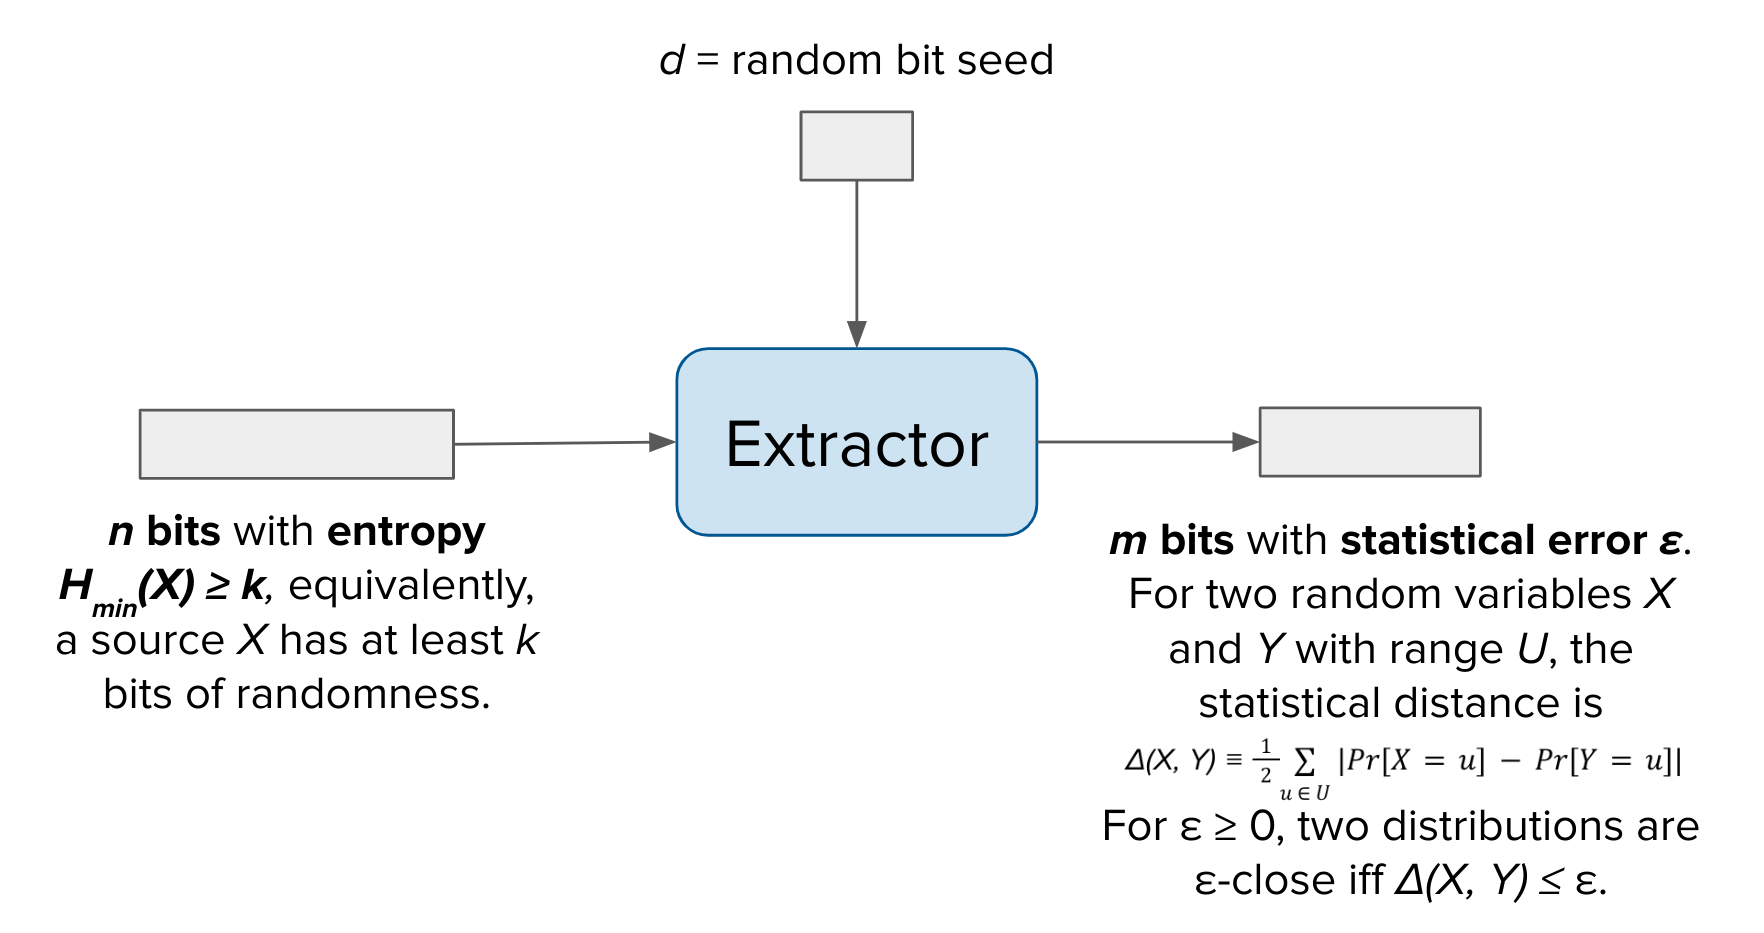
\includegraphics[scale=0.18]{Images/CC_extractor_updated.png}
    \caption{Classical-to-classical (seeded) randomness extractor}
    \label{fig:ExtractorDiagram}
\end{figure}

Recall that our motivation for extractors was to simulate randomization given only a weak random source, or without a seed. If the seed is of logarithmic length, i.e. $d=O(\log n)$, then instead of selecting it randomly we can enumerate all possibilities for the seed and take a majority vote. In summary, the randomness used for seeds can be eliminated by running all the possible seeds and taking the majority value. This is formally defined by the following lemma. 

\begin{lemma}
    Let $A(w,r)$ be a randomized algorithm such that $A(w,U_m)$ has error probability at most $\gamma$, and let $\ibeext:\{0,1\}^n \times \{0,1\}^d \rightarrow \{0,1\}^m$ be a $(k,\varepsilon)$ extractor. Define $A' = {\rm majority}_{y \in \{0,1\}^d} \{A(w, \ibeext(x,y))\}$. Then for every $k$-source\footnote{A random variable $X$ is $k$-source if $H_{\min}(X) \geq k$.} $X$ on $\{0, 1\}^n$, $A'(x, X)$ has error probability of at most $2(\gamma + \varepsilon)$.
\end{lemma}

As stated above, we wish to extract randomness from weak random source $X$ without any additional uniform randomness. Therefore it follows that we want to keep $Y$ as small as possible, even though $X$, and $k$, could be very large. In other words, we would like a long output (i.e. large $m$) using a short seed (i.e. small $d$). This motivates the following definition of strong extractors. 
% The advantage of strong extractors is that the output is close to the uniform distribution even if the value of $U_d$ is known.

\begin{definition}\normalfont{\textbf{(Strong Extractor)}}
    Extractor $\ibeext : \{0, 1\}^n \times \{0, 1\}^d \rightarrow \{0,1\}^m$ is a strong $(k, \varepsilon)$-extractor if for every $k$-source $X$ on $\{0,1\}^n$, $(U_d, \ibeext(X,U_d)$ is $\varepsilon$-close to $(U_d, U_m)$. Equivalently, $\ibeext'(x,y) = (y, \ibeext(x,y))$ is a standard ($k, \varepsilon$)-extractor.
\end{definition}

Before we discuss the explicit construction of a strong extractor, we revisit the question of why the min-entropy is a correct measure to quantify the amount of randomness that can be extracted from a given source? Informally, we can argue that the min-entropy is an upper bound on the amount of randomness that can be extracted: there does not exist any strong extractor that has an output length more than $H_{\min}(X)$. To understand this, first recall that $H_{\min}(X) = - \log P_{\text{guess}}(X)$. Suppose that we now apply some function $f$ to source $X$, then how difficult is it to guess $f(X)$, i.e., what is $P_{\text{guess}}(f(X))?$. Clearly, we can guess $f(X)$ by first guessing $X$ and then applying $f$ to our guess. Thus, we get $P_{\text{guess}}(f(X))\geq P_{\text{guess}}(X)$. However, this is equivalent to
\[H_{\min}(f(X))\leq H_{\min}(X).\]
In other words, this also means that the output of the extractor $\ibeext$ is obtained as a function
$f(X) = \ibeext(X,y)$, for a fixed seed $y$, must have min-entropy at most $H_{\min}(X)$. Thus, the output $\ibeext(X,y)$ can be uniform on at most $H_{\min}(X)$ bits.
How about a converse: does there exist a strong extractor that can extract approximately $H_{\min}(X)$ bits from any $k$-source X? The answer to this question is yes.

We now explore a construction of randomness extractors that achieves well-performing parameters for this application, the 2-universal extractor. Our goal for our parameters is large $m$, or extracting as much randomness as possible, using the smallest possible seed and error, or small $d$ and $\varepsilon$. First, we must define a 2-universal family.
\begin{definition}\normalfont{\textbf{(2-universal family)}}
    A family of hash functions $\mathcal{F} = \{f:\{0,1\}^n \rightarrow \{0,1\}^m\}$ is called \textit{2-universal} if for every two strings $x,x' \in \{0,1\}^n$ with $x \neq x'$, and any two $z, z' \in \{0,1\}^m$, we have
    \[
        \Pr_{f \in \mathcal{F}}[f(x) = z \oplus f(x') = z'] = \frac{1}{2^{2m}}.
    \]
\end{definition}

Using 2-universal families, we are able to define 2-universal extractors as follows.
\begin{definition}\normalfont{\textbf{(2-universal extractor)}}
    Let $\mathcal{F} = \{f_y:\{0,1\}^n \rightarrow \{0,1\}^m, y \in \{0,1\}^d\}$ be a 2-universal family of hash functions such that $|\mathcal{F}| = 2^d$. The associated 2-universal extractor is 
    \[
        \ibeext_{\mathcal{F}}:\{0,1\}^n \times \{0,1\}^d \rightarrow \{0,1\}^m, \ibeext_{\mathcal{F}}(x,y) = f_y(x).
    \]
\end{definition}
Conceptually, consider $\ibeext_{\mathcal{F}}$ as using a seed $y$ to select a function from the family $\mathcal{F}$ uniformly at random and returning the output of the function when evaluated on the source $X$. To evaluate how good this extractor is, we use the leftover hash lemma (insert reference), which is defined as follows.
\begin{definition}\normalfont{\textbf{(Leftover hash lemma)}}
    Let $n$ and $k \leq n$ be arbitrary integers, $\varepsilon > 0$, $m = k - 2\log(\frac{1}{\varepsilon})$, and $\mathcal{F} = \{f: \{0,1\}^n \rightarrow \{0,1\}^m\}$ a 2-universal family of hash functions. Then the 2-universal extractor $\ibeext_{\mathcal{F}}$ is a $(k,\varepsilon)$-strong seeded randomness extractor.
\end{definition}
Due to page limit restrictions, for the leftover hash lemma proof, we refer the reader to \cite{tudelftQC}.

%%% Hey Kyle, Samin wrote the discussion. Could you go through it and check if it looks good?

\section{Preliminaries}
In this section, we recall the basic \textit{Dirac} notation of quantum information science which we will use throughout this article. We refer the reader to \cite{wilde2013quantum,nielsen2002quantum} for additional reading in quantum computation and quantum information. The Dirac notation represents a vector using the left vertical bar and the right angle bracket, known as \emph{ket} vector. Thus it can be understand by the following map:
$x \rightarrow \ket{x}$ for any index $x$. The conjugate transpose of the ket vector $\ket{x}$ is known as \emph{bra} vector and denoted as $\bra{x} = \ket{x}^{\dagger}$. In other words, the $\ket{x}$ in Dirac notation represents the column vector, whereas $\bra{x}$ represents the row vector (conjugate transpose of the column vector $\ket{x}$).

%%%%%%%%%%%%%%%%% Mathematical Background %%%%%%%%%%%%%%%%% 
\subsection{Mathematical Background}
 In this subsection, we go through some of the mathematical tools that will be required to understand the QC and QQ randomness extractor. We restrict ourselves to definitions and a few important properties; for detailed understanding, we refer the reader to cite \ {wilde2013quantum, nielsen2002quantum}.
 
 \begin{definition}\textbf{(Conjugate Transpose)}
The \emph{conjugate transpose} or \emph{Hermitian transpose} of a $m\times n$ complex matrix $A$ is a $n\times m$ matrix $A^\dagger$ obtained by transposing $A$ followed by applying complex conjugate on each entry or vice versa, i.e., $A^\dagger = \bar{(A^\text{T})} = (\bar{A})^{\text{T}}$. 

For real matrices, the conjugate transpose is just the transpose, $A^{\dagger} =A^{\text{T}}$.
\end{definition}
 
\begin{definition}\textbf{(Hilbert Space)} A Hilbert space is a complex vector space $\calH$ with an inner product   $ \bra{x}\ket{y} \equiv \langle  x | y \rangle $, where $x,y \in \calH$, such that the norm defined as $\norm{x} = \sqrt{\langle  x |x \rangle}$ make $\calH$ a complete metric space. It allows generalizing the methods of linear algebra and calculus from (finite-dimensional) Euclidean vector spaces to spaces that may be infinite-dimensional.
\end{definition}

\begin{definition}\textbf{(Linear Operator)}
A \emph{linear operator} A on a Hilbert space $\calH$ is a mapping $A:\calH\rightarrow\calH$ such that
\[A\left(\sum_i \alpha_i \ket{x_i}\right) = \sum_i \alpha_i A\ket{x_i}.\]

The set of linear operators is denoted as $\calL(\calH,\calH)$.
\end{definition}

\begin{definition}\textbf{(Trace of Linear Operator)}
The trace of an operator $A \in \calL(\calH,\calH)$ is defined as
\[\Tr(A) = \sum_i \bra{i}A\ket{i},\]

where $\set{\ket{i}}$ is any orthonormal basis of $\calH$.
\end{definition}

\begin{definition}\textbf{(Hermitian Operator)}
A \emph{linear operator} $A \in \calL(\calH,\calH)$ is \textit{hermitian} if $A^\dagger = A$. 
\end{definition}

\begin{definition}\textbf{(Positive Semi-Definite Operator)} A hermitian operator $A$ is positive semi-definite if all its eigenvalues are non-negative. 
\end{definition}

\begin{definition}\textbf{(Adjoint)} The \emph{adjoint} or \emph{Hermitian conjugate} of the operator $A \in \calL(\calH,\calH)$ is a \emph{unique} linear operator $A^{\dagger} \in \calL(\calH,\calH)$ such that for all $\ket{x},\ket{y} \in \calH,$ 
\[\bra{x} \left(A\ket{y}\right) = \left(A^\dagger\ket{x}\right)^\dagger\ket{y}.\]
\end{definition}

% \begin{itemize}
%     \item 2.1.2 Some Notation about semi-definite operators and $\sigma$-weighted $\alpha$-norms
%     \item von Neumann algebra
% \end{itemize}

In the following subsections, we go through the mathematical framework of quantum mechanics, namely, formalism of quantum states and time-evolution of quantum states. We refer the reader to \cite{sakurai1995modern, zettili2003quantum, griffiths2018introduction} for additional understanding of concepts in quantum mechanics.
\subsection{Quantum States}
\begin{definition}\textbf{(Quantum System)} A Quantum System is a complex vector space with an inner product, i.e., a Hibert space $\calH$. By following the convention in quantum cryptography, we assume all Hilbert Space is finite-dimensional. 
\begin{example}
    The simplest quantum system is a \textit{qubit} or \textit{quantum bits}, which is a two-dimensional quantum system. 
\end{example}
\end{definition}

\begin{definition}\textbf{(Quantum States)}
Let $|A|$ be the dimension of a quantum system $A$ acting on Hilbert space $\calH_A$, and $\mathcal{L}(A)$ denote the set of linear operators on system $A$. We define a \emph{quantum state} on system $A$ as $\rho_{A} \in \mathcal{S}(A)$ where $\mathcal{S}(A) = \{ \sigma_{A} \in \mathcal{L}(A) | \sigma_{A} \geq 0$, $\Tr(\sigma_A) = 1\}$, i.e., a quantum state is a unit-trace and positive semi-definite linear operator on $\calH_A$. 
\end{definition}
\begin{example}
    Let $\ket{0}$ and $\ket{1}$ form an orthonormal basis for a qubit system $\calH_2$. Then any arbitrary qubit state $\rho_2$ can be written as $\ket{\psi}\bra{\psi}$ where $\ket{\psi} \in \calH_2$ is an arbitrary \textit{superposition} of the basis state, i.e., 
$\ket{\psi} = \alpha\ket{0} + \beta \ket{1}$
such that $\alpha$ and $\beta$ are complex numbers and $|\alpha|^2 + |\beta|^2=1$. After simplifying, $\rho_2 = |\alpha|^2 \ket{0}\bra{0} + \alpha \bar{\beta}\ket{0}\bra{1} + \beta \bar{\alpha}\ket{1}\bra{0} + |\beta|^2 \ket{1}\bra{1}$. We can also write $\rho_2$ in matrix form w.r.t basis $\set{\ket{0}, \ket{1}}$ as
\[\rho_2 =  \begin{pmatrix}
|\alpha|^2 & \alpha \bar{\beta}\\
\beta \bar{\alpha} & |\beta|^2
\end{pmatrix}.\]
\end{example}


We call $\rho_A$ a \emph{pure state}, if it has rank 1.
If $\Tr(\rho_A) \leq 1$, we call $\rho_A$ a sub-normalized state. We use the notation $\calS_{\leq}(A)$ to represent a collection of sub-normalized states of the system $A$. For the rest of the paper, the term \emph{state} is referred to sub-normalized  state unless otherwise specified.
\begin{definition}\textbf{(Multipartite Quantum States)}
We define a (separable) multipartite system\footnote{A multipartite system $A_1A_2\cdots A_n$ is called a \textit{separable} system if it can be written as tensor product of individual systems, i.e., $A_1A_2\cdots A_n = A_1 \otimes A_2\otimes \cdots \otimes A_n$, otherwise the multipartite system is called \emph{entangled} system. We will mainly consider the bipartite state, where two systems $A_1$ and $A_2$ are combined using the tensor product and written as $A_1A_2 = A_1 \otimes A_2$} ${A_1A_2\cdots A_n}$ by the \emph{tensor product} of individual quantum systems $A_1, A_2, \cdots, A_n$ acting on the Hilbert space $\calH_{A_1A_2...A_n}$, where 
$$\calH_{A_1A_2...A_n} = \calH_{A_1} \otimes \calH_{A_2}, ...,  \otimes \calH_{A_n}.$$
Then, a \textit{multipartite} quantum state $\rho_{A_1A_2\cdots A_n} \in \calS_{\leq}(A_1A_2\cdots A_n)$. 
\end{definition}

If $n=2$, the quantum state $\rho_{A_1A_2}$ is known as \emph{bipartite} quantum state. The quantum state of the subsystem $A_1$ is defined as $\rho_{A_1} = \Tr_{A_2}[\rho_{A_1A_2}]$, where $\Tr_{A_2}$ is the partial trace\footnote{For brief understanding partial trace information please see: \href{https://en.wikipedia.org/wiki/Partial\_trace}{Partial Trace (wikipedia)}} on system $A_2$. In other words, the quantum state of the subsystem $A_1$ is the restriction of $\rho_{A_1A_2}$ onto $\calH_{A_1}$. Similarly, the quantum state of the subsystem $A_2$ can be obtained by partial tracing the system $A_2$.  

\begin{definition}\textbf{(Purification)}
\emph{Purification} is the completion of a quantum system by adding a purifying or reference system $R$. Let $\rho_A \in \mathcal{S}_{\leq}(A)$ be a sub-normalized state. 
% A \emph{purification} of $\rho_A$ is a pure bipartite state $\ket{\rho_A}$ defined as a triple ($\pi, \calH, |\mathcal{E}\rangle$), where $\pi$ is the representation of $\calH_A$ on a Hilbert Space $\calH$, and $\mathcal{E} \in \calH_A$ such that
A \emph{purification} of $\rho_A$ is a pure bipartite state $\ket{\rho}_{AR}$ on the purifying system $R$ and the original system $A$ such that
$$\rho_A = \Tr_R(\ket{\rho}\bra{\rho}_{AR}).$$
% We call $\pi(\calH_A)$ the \emph{principle} and $\pi(\calH_A)'$ the \emph{purifying system}. 
\end{definition}
Purification is not unique. However, all possible purifications of a quantum state $\rho_A$ are related by an isometry \footnote{Given two Hilbert spaces $\mathcal{H}_1$ and $\mathcal{H}_2$ with dim($\mathcal{H}_1$) $\leq$ dim($\mathcal{H}_2$), an isometry $V$ is a linear map from $\mathcal{H}_1$ to $\mathcal{H}_2$ such that $V^\dag V = \I_{\mathcal{H}_1}$ \cite{wilde2013quantum,nielsen2002quantum}.} acting on the reference system $R$ \cite[Theorem 5.1.1]{wilde2013quantum}.

\begin{definition}\textbf{{(Classical States)}}
For some set $\mathcal{X}$, let $\{|x\rangle \}_{x \in \mathcal{A}}$ be the orthogonal basis of a Hilbert space $\calH_X$, where each basis basis vector $|x\rangle$ corresponds to a particular element $x \in \mathcal{X}$. A \emph{classical state}, or a c-state, $\rho_X$ defined using the distribution $P_X$ over $\mathcal{X}$ as follows: 
$$\rho_X = \sum_{x \in \mathcal{X}}P_X(x)|x \rangle \langle x|.$$
\textbf{(Classical-Quantum States)} The joint system of a classical system $X$ and a quantum system $A$ is defined as
\[
  \rho_{XA} = \sum_{x \in \mathcal{X}}P_X(x)
    \underbrace{\ket{x}\bra{x}_X}_\text{classical} \otimes \underbrace{\rho^x_A}_\text{quantum},
\]
\end{definition}
and such states are called \emph{classical-quantum} states, or cq-states. In general, when a multipartite state is partly classical and partly quantum, we use $c$ and $q$ to label the classical and quantum systems, respectively.

\begin{example} In quantum cryptography, we often encounter cq-states. Suppose Alice tosses a fair coin, and if the head appears, she prepares a $\ket{0}$ state and $\ket{1}$ otherwise. Alice then transmits her state to Bob. Thus, if Alice state is $\ket{0}$ or $\ket{1}$, then Bob will receive $\rho_0^B$ or $\rho_1^B$, respectively. The joint state of Alice and Bob can be written as a cq-state of the form:
\[\rho_{AB} =  \frac{1}{2}  \sum_{x\in \set{0,1}} \ket{0}\bra{0}_A \otimes \rho_x^B.\]
\end{example}


%%%%%%%%%%%%%%%%% Quantum Operations %%%%%%%%%%%%%%%%% 
\subsection{Quantum Operations} 
\begin{definition}\textbf{(Quantum Measurement)}
Consider a set of positive semi-definite operators $\set{M_x^{A_2}}_{x\in \calX}$ acting on system $A_2$ such that $\sum_x M_x^{A_2} = \I_{A_2}$. For a bipartite system $A_1A_2$, a \emph{measurement map} on the system $A_2$ is defined as $\mathcal{T}_{A_1A_2 \rightarrow A_1}:\mathcal{L}(A_1A_2) \rightarrow \mathcal{L}(A_1)$,
$$\mathcal{T}(\I_{A_1} \otimes M_x^{A_2})_{A_1A_2 \rightarrow A_1} = \sum_{a_1a_2} \langle a_1a_2|(\I_{A_1} \otimes M_x^{A_2})|a_1a_2 \rangle |a_1\rangle \langle a_1|$$
where $\{|a_1\rangle\}, \{|a_2\rangle\}$ are standard orthogonal bases of $A_1, A_2$ respectively. The subscript $x$ is used as a label for measurement outcomes. \autoref{fig:measurement} provides the schematic of a quantum measurement. The probability of observing $x$ on system $A_2$ is given as $p_x^{A_2} = \langle a_1a_2|(\I_{A_1} \otimes M_x^{A_2})|a_1a_2 \rangle = \langle a_2|M_x^{A_2}|a_2 \rangle = \Tr(M_x^{A_2}|a_2 \rangle \langle a_2|)$\footnote{The interpretation of inner product as probability follows from \textit{Born rule}}.

The set of positive semi-definite operators $\set{M_x^{A_2}}_{x\in \calX}$ referred as positive valued measurements (POVMs). In quantum information theory and cryptography, we are mostly interested in the probabilities of measurement outcomes but not the output state after measurement. Thus, POVMs provide simpler expressions for finding probabilities of outcomes. 
% Note that the outcome of the measurement map is classical in the basis $\{|a_1 \rangle\}$ on $A_1$.
\end{definition}
\begin{figure}[!htb]
    \centering
    
\includegraphics[scale=0.45]{Images/measurement.png}
    \caption{Quantum measurement}
    \label{fig:measurement}
\end{figure}
\begin{example}
    Consider a distribution $p_X$ and the classical state $\rho_X = \sum_{x} p_X(x) \ket{x}\bra{x}$. If we
measure $\rho_X$ in the standard basis, i.e. $\set{\ket{x}}$, with associated POVM $M_x = \ket{x}\bra{x}$, we
obtain outcome $x$ with probability
$\Tr(M_x\rho_X) = \Tr(\ket{x}\bra{x} \rho_x) = \bra{x}M_x\ket{x}p_X(x) = p_{X}(x)$.
Thus, we observe that $\rho_X$ indeed captures the classical distribution given by the probabilities $p_x$. 
\end{example}
\begin{definition}\textbf{(Unitary Evolution)} The evolution of a quantum state is described by a \textit{unitary} transformation. Suppose a  \emph{unitary operator}\footnote{Given two Hilbert spaces $\mathcal{H}_1$ and $\mathcal{H}_2$ with dim($\mathcal{H}_1$) $=$ dim($\mathcal{H}_2$), an unitary $U$ is a linear map from $\mathcal{H}_1$ to $\mathcal{H}_2$ such that $V^\dag V = V V^\dag = \I_{\mathcal{H}_1}$ \cite{wilde2013quantum,nielsen2002quantum}.} $U$ is applied to system $A_1$ of $\rho_{A_1A_2}$. Then the evolved quantum state can be written as
$$\rho'_{A_1A_2} = U_{A_1}\rho_{A_1A_2}U^{\dag}_{A_1} = (U \otimes \I_{A_2})\rho_{A_1A_2}(U \otimes \I_{A_2})^{\dag},$$
\end{definition}
where $\I_{A_2}$ denotes the identity in $\mathcal{L}(A_2)$.
\begin{definition}\textbf{(Identity Channel)}
For quantum systems $A_1, A_2$ with orthogonal bases 
$\{|i \rangle_{A_1}\}^{d}_{i=1}, \{|i \rangle_{A_2}\}^{d}_{i=1}$,
the \emph{identity channel} $\I$, from $\mathcal{L}(A_1)$ to $\mathcal{L}(A_2)$ with respect to these bases is denoted by $\I_{A_1 \rightarrow A_2}$, where $\I_{A_1 \rightarrow A_2}(|i\rangle \langle j|_{A_1}) = |i\rangle \langle j|_{A_2}$.
\end{definition}
\begin{definition}\textbf{(Quantum Channel)}
A linear map $\mathcal{E}_{A_1 \rightarrow A_2}: \mathcal{L}(A_1) \rightarrow \mathcal{L}(A_2)$ is a quantum channel if it satisfies the following conditions: 
\begin{itemize}
    \item $ \Tr(\mathcal{E}_{A_1 \rightarrow A_2})(\rho_{A_1}) = \Tr(\rho_{A_1})$, i.e., trace-preserving and
    \vspace{-2pt}
    \item $ (\I_A \otimes \mathcal{E}_{A_1 \rightarrow A_2})(\I_A \otimes \rho_{A_1}) \geq 0$ for all $\rho_{A_1} \geq 0$, i.e., completely positive.
\end{itemize} In other words, a \emph{quantum channel} is a linear, completely positive and trace-preserving map.
\end{definition}

We conclude the brief discussion about  the mathematical framework of quantum mechanics. \autoref{fig:qip} summarizes a quantum information processing task, which includes $(i)$ the preparation of quantum states, i.e., encoding, $(ii)$ performing some quantum operation, for example, passing the input quantum state through a quantum channel, and $(iii)$ decoding the classical outcome by performing a quantum measurement. 
\begin{figure}[!htb]
    \centering
    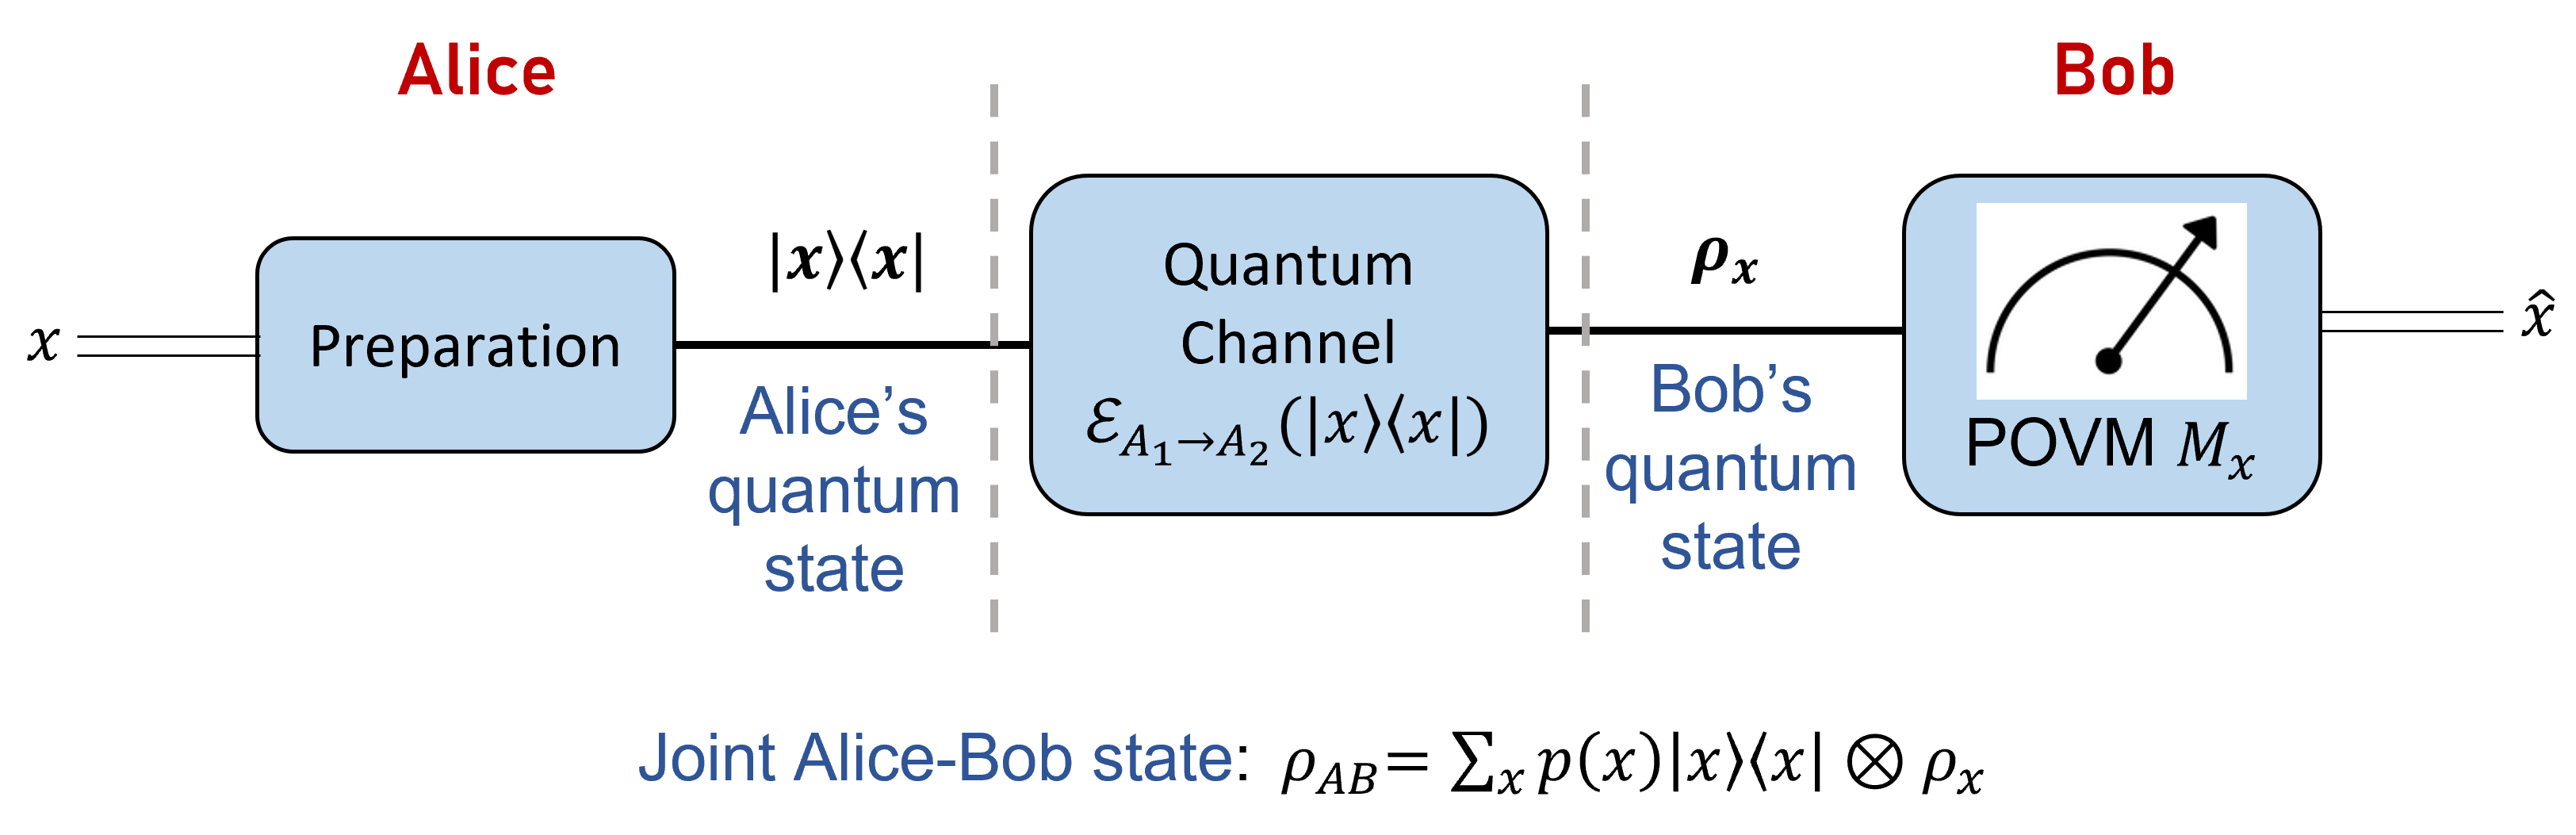
\includegraphics[scale=0.45]{Images/qip.png}
    \caption{Schematic of a quantum information processing task.}
    \label{fig:qip}
\end{figure}

In the following subsections, we discuss the statistical distance between two quantum states, i.e., how to measure the closeness of two quantum states and quantum information quantities. We refer the reader to \cite{wilde2013quantum, nielsen2002quantum} for additional understanding of distance and information measures. 
%%%%%%%%%%%%%%%%% Distance Measures %%%%%%%%%%%%%%%%% 
\subsection{Distance Measures} Distance measure quantifies the closeness of quantum states. In this subsection, we discuss two well-studied distance measures for sub-normalized quantum states, namely, $(i)$ \emph{trace distance} and $(ii)$ \emph{purified distance}. We begin by defining the trace distance followed by the purified distance. We further provide brief intuition about these distance measures. However, for detailed discussion, we refer to \cite{berta2013quantum}.
\begin{definition} \textbf{(Trace Norm)}
The trace norm or Schatten 1-norm $\norm{\rho}_1$ of a quantum state $\rho$ is defined as 
\[\norm{\rho}_1 = \Tr\set{\sqrt{\rho^\dagger \rho}}.\]
\end{definition}
The trace norm induces a distance measure between quantum states called \emph{trace distance}.
\begin{definition}\textbf{(Trace Distance)} Given any two quantum states $\rho$ and $\sigma$, the trace distance between them is as follows:
\[\norm{\rho-\sigma}_1.\]
\end{definition}
For any two quantum states $\rho$ and $\sigma$, the following bounds hold for the trace distance:
\[0\leq \norm{\rho-\sigma}_1 \leq 2.\]
The trace distance attains a lower bound when two quantum states are equivalent, i.e., there exists no measurement that can distinguish $\rho$ and $\sigma$. The trace distance attains the upper bound when $\rho$ and $\sigma$ have support on orthogonal subspaces, i.e., there exists a measurement that can distinguish $\rho$ and $\sigma$.

\begin{definition}\textbf{(Generalized Fidelity)} The generalized fidelity between two quantum states $\rho$ and $\sigma$ is defined as
\[\bar{F}(\rho,\sigma) = F(\rho,\sigma) + \sqrt{(1-\Tr(\rho)\Tr(\sigma))},\]
where $F(\rho,\sigma) = \norm{\sqrt{\rho}\sqrt{\sigma}}_1$ is the notion of fidelity between normalized quantum states. Note that if either of the quantum states is normalized, then generalized fidelity is the same as the fidelity, i.e., $\bar{F}(\rho,\sigma) = F(\rho,\sigma)$. 
\end{definition}

\begin{definition}\textbf{(Purified Distance)} The purified distance between two quantum states $\rho$ and $\sigma$ is defined as 
\[P(\rho,\sigma) = \sqrt{1-\bar{F}(\rho,\sigma)}.\]
\end{definition}
The \textit{purified distance} is a metric on the set of sub-normalized quantum states. The purified distance and trace distance are closely related as, for any two states $\rho,\sigma$, we have \cite{tomamichel2012framework},
\[\frac{1}{2}\norm{\rho-\sigma}_1 \leq P(\rho,\sigma) \leq \sqrt{2\norm{\rho-\sigma}_1}.\] 

\begin{definition}\textbf{($\boldsymbol{\varepsilon}$-quantum ball)} Let $\calH_A$ be a Hilbert space. The $\varepsilon$-quantum ball around a quantum state $\rho_A \in \calS_{\leq}(A)$ of the system $A$ is defined as the collection of quantum states $\set{\sigma_A \in \calS_{\leq}(A)}$ such that the purified distance between $\rho_A$ and $\sigma_A$ is not more than $\varepsilon$, i.e.,
\[\calB^{\varepsilon}(\rho_A) = \set{\sigma_A \in \calS_{\leq}(A) : P(\rho_A,\sigma_A) \leq \varepsilon}.\]
\end{definition}
We use the above definition to describe the notion of smooth conditional $\min$-entropy of a quantum system in the next section.

\subsection{Information Quantities}
The term ``information'' in the context of information theory is a measure of how much we can learn from the outcome of a random experiment. Information can be classical, quantum, or both depending on the physical source of information. For example, measuring the position of an electron  carries \emph{quantum information}, whereas flipping a coin carries \emph{classical information}.  The fundamental information measure in classical and quantum information theory is \emph{entropy}. Entropy is the expected amount of information contained in an outcome of a random experiment \cite{shannon1948mathematical}. In this section, we define the various entropy measures that are required to provide the information-theoretic operational interpretations of randomness extractors. We discuss some of their mathematical properties. However, we exclude the proofs; for further understanding, we refer to \cite[Ch-10,11]{wilde2013quantum}. We start by defining quantum entropy, also known as \textit{Von Neumann entropy} for general quantum systems. Furthermore, we define quantum (Von-Neumann) conditional entropies. We then discuss the condition min-entropy of a bipartite quantum system analogous to classical conditional min-entropies. Finally, we conclude the subsection with the definition of smooth conditional min-entropy, which is helpful in quantum cryptography, especially in the context of entropic uncertainty, noisy storage model, and privacy amplification \cite{Vazirani2014FullyDQ}.

\begin{definition}\textbf{(Von Neumann Entropy)} The entropy of a quantum state $\rho_A \in \calS_{\leq}(A)$ is defined as
\[H(A)_\rho = -\Tr(\rho_A \log \rho_A) \footnote{All logarithms are base 2 unless specified.}
.\]
% Note for a classical state, $\rho_X$, $H(A)_\rho = H(X)$, i.e., Von Neumann entropy is given by Shannon entropy.
\end{definition}

\begin{definition}
\textbf{(Conditional Von Neumann Entropy)} The conditional entropy of quantum system $A$ given $B$ for bipartite quantum state $\rho_{AB} \in \calS_{\leq}(AB)$ is defined as
\[H(A|B)_{\rho} = H(AB)_{\rho} - H(B)_{\rho},\]
where $H(AB)_{\rho} = -\Tr(\rho_{AB} \log \rho_{AB})$ is the Von Neumann entropy of the bipartite state $\rho_{AB}$.
\end{definition}

%%% Quantum Mutual Information
% \begin{definition}(Quantum Mutual Information)
% The mutual information between quantum systems $A$ and $B$ for bipartite quantum state $\rho_{AB}$ is defined as 
% \[I(A;B)_{\rho} = H(A)_{\rho} + H(B)_{\rho} - H(AB)_{\rho}.\]
% \end{definition}

We provide the definitions of the min- and max-based information measures analogous to Def. \ref{def:min_entropy}. 


\begin{definition}
\textbf{(Min-Conditional Entropy)} The min-conditional entropy of a bipartite quantum state $\rho_{AB}$ with respect to a quantum state $\sigma_B$ is defined as 
\[H_{\min}(A|B)_{\rho|\sigma} = \max\set{\lambda \in \R : 2^{-\lambda}\cdot \I \otimes \sigma_B \geq \rho_{AB}}\]
\end{definition}

\begin{definition}
\textbf{(Conditional Min-Entropy) }The conditional min-entropy of a bipartite quantum state $\rho_{AB}$ is defined as 
\[H_{\min}(A|B)_{\rho} = \max_{\sigma_B \in \calS(B)} H_{\min}(A|B)_{\rho|\sigma}\]
\end{definition}

To interpret a conditional information measure, suppose Alice and Bob want to share a bipartite quantum state $\rho _{AB}$. Alice and Bob have access to systems $A$ and $B$, respectively. The conditional entropy measures the average uncertainty Bob has about Alice's state upon sampling from his own system.
 
The above-mentioned entropies have operational interpretation only in an independent and identically (IID) distributed asymptotic setting. Therefore, for an operational characterization of a generalized quantum system, we need a notion of \textit{smooth entopies} \cite{tomamichel2012framework}. 

%\textbf{Smooth Conditional Min-Entropy}
 
\begin{definition}\textbf{(Smooth Conditional Min-Entropy)} Let $\rho_{AB} \in \calS_{\leq}(AB)$ be a quantum state and $\varepsilon \geq 0$. The $\varepsilon$-smooth conditional min-entropy of $A$ given $B$ is defined as
\[H_{\min}^{\varepsilon}(A|B)_\rho = \sup_{\sigma_{AB} \in \calB^{\varepsilon}(\rho_{AB})} H_{\min}(A|B)_{\sigma}.\]
\end{definition}

% Smooth entropies emerge from their non-smooth counterparts by a maximization and minimization, respectively, over states close with respect to a suitable distance measure. The choice of the distance measure influences the properties of the smooth entropies crucially. Here, we follow Tomamichel [Tom12], and define the smooth entropies using ε-balls with respect to the purified distance. For ω ∈S≤(M) and ε≥0, we define Bε M(ω) = {σ ∈ S≤(M) : PM(ω,σ) ≤ ε} . (2.45) The set Bε M(ω) is referred to as the smoothing set, and ε is called the smoothing parameter. In the following, we often omit the indication of the von Neumann algebra Mwhenever it is clear from the context.

\section{Quantum-to-Classical Randomness Extractors}\label{sec:qc_ext}
In this section, we study quantum-to-classical randomness extractors (QC-extractors). The main objective of this section is to answer the following question: how can we extract classical randomness from a physical (quantum) source $\rho_{AE}$ by performing measurements on the quantum state $\rho_A$? Here, $A$ is the accessible quantum source, and $E$ is the environment or eavesdropper correlated with $A$. Similar to the study of classical extractors in \autoref{sec:c_ext}, we want to extract randomness from a quantum source given  min-entropy $H_{\min}(A|E)_\rho \geq k$. It is worth noting that, unlike the classical world, quantum mechanics does allow for the generation of true randomness in case we can prepare the desired quantum source. For example, if we could prepare the state $\ket{+} = {1/\sqrt{2}}(\ket{0} + \ket{1})$ or $\ket{-} = {1/\sqrt{2}}(\ket{0} - \ket{1})$ and measure it in the computational basis\footnote{$\set{\ket{0}, \ket{1}}$ is known as the computational basis of a qubit system, whereas $\set{\ket{+}, \ket{-}}$ is known as Hadamard basis of a qubit system}, i.e., $M_0 = \ket{0}\bra{0}$ and $M_1 = \ket{1}\bra{1}$. Then, we get a \textit{true} random coin. However, this would require preparing the exact source of this form. In general, we want to construct a QC extractor that works for any unknown quantum source as long as it has a sufficiently high min-entropy.

To understand the definition of quantum extractors, consider a classical extractor as a family of permutations acting on the possible values of the source such that it applies a typical permutation from the family to the input for any probability distribution on input bits strings with high min-entropy, which induces an almost uniform probability distribution on a prefix of the output. We define a QQ-extractor similarly in the way that lets the operations be general unitary transformations and the input of the extractor be quantum.

\begin{definition}\textbf{(QQ-extractor \cite{Berta_2014})} 
    Let $A = A_1A_2$ (entangled system) with $n = \log |A|$, define the trace-out map $\Tr_{A_2} : \mathcal{L}(A) \to \mathcal{L}(A_1)$ by $\Tr_{A_2}(\cdot) = \sum_{a_2} \langle a_{2}|(\cdot)|a_{2} \rangle$, where $\{|a_2 \rangle \}$ is an orthonormal basis of $A_2$. For $k \in [-n, n]$ and $\epsilon \in [0,1]$, a $(k, \epsilon)$-QQ-extractor is a set $\{U_1, \dots, U_L\}$ of unitary transformations on $A$ such that for all states $\rho_{AE} \in \mathcal{S}(AE)$ satisfying $H_{min}(A|E)_{\rho} \geq k$, we have 
    
    \begin{align*}
        \frac{1}{L} 
        \sum_{i = 1}^{L} 
        \left\|\Tr_{A_2}(U_{i} \rho_{AE} U_{i}^{\dagger}) - \frac{\I_{A_{1}}}{|A_{1}|} \otimes \rho_{E}\right\|_{1} \leq \epsilon. 
    \end{align*}
    
    where $\log L$ is called the seed size of the QQ-extractor.
\end{definition}

More often than not, we only need a quantum extractor as it is usually sufficient to extract random classical bits. Doing so is much easier than obtaining random qubits. This motivates our need for quantum-classical extractors, where the output system $M$ is measured in the computational basis. Generally, our QC-extractor can be represented as given in \autoref{fig:qc_extractor}. We take a quantum input system with our seed and mix it. Mixing is done with the unitary operation, where we take one basis of the Hilbert space of the quantum system and rotate it into another Hilbert space. After mixing, we use the process of measuring and discarding to generate our classical output system. For that, first, we define the measurement map for $\calH_M \subseteq \calH_N$ as $\calT_{N \to M}: \calH_N \rightarrow \calH_M$,
\begin{align*}
    \calT_{N \to M}(\cdot) = \sum_{m, m'} \bra{mm'} (\cdot) \ket{mm'} \ket{m} \bra{ m }_{M}
    \label{eq:measurement_map}
\end{align*} 
where $\set{ \ket{mm'}}, \set{\ket{m}}$ are orthonormal bases of $\calH_{N}, \calH_{M}$, respectively. We can also observe this map as tracing out $N / M$, and measuring the remaining system $M$ in the basis $\set{\ket{m}}$. Using the above map, we will define quantum-classical min-entropy extractors against quantum side information.

\begin{definition}\textbf{(QC-extractor \cite{Berta_2014})}\label{def:measurement_map}
    Let $A = A_{1} \otimes A_{2}$ (separable system) with $n = \log |A|$. Define the \emph{measurement map} $\calT_{A \to A_{1}}: \calL(A) \to \calL(A_{2})$ by 
    \begin{align}
        \calT_{A \to A_{1}}(\cdot) 
        &= \sum_{a_{1} a_{2}} \bra{a_{1} a_{2}} (\cdot) \ket{a_{1} a_{2}} \ket{a_{1}} \bra{a_{1}},
    \end{align}
    where $\{\ket{a_{1}}\}, \{\ket{a_{2}}\}$ are standard orthonormal bases for $A_{1}, A_{2}$ respectively. 
    
    For $k \in [-n, n]$ and $\varepsilon \in [0, 1]$, a \emph{$(k, \varepsilon)$-QC-extractor} is a set $\{U_{1}, \dots, U_{L}\}$ of unitary transformations on $A$ such that for all states $\rho_{AE} \in \calS(AE)$ satisfying $\Hmin(A|E)_{\rho} \ge k$, we have 
    \begin{align*}
        \frac{1}{L} 
        \sum_{i = 1}^{L} 
        \left\|\calT_{A \to A_{1}}(U_{i} \rho_{AE} U_{i}^{\dagger}) - \frac{\I_{A_{1}}}{|A_{1}|} \otimes \rho_{E}\right\|_{1} \le \eps. 
    \end{align*}
    $\log L$ is called the \emph{seed size} of the QC-extractor. 
\end{definition}

The reason we use this definition is that we want the output of the extractor to be determined by the source and the choice of the seed. In the quantum setting, a natural way of translating this requirement is by imposing that an adversary holding a system that is maximally entangled with the source can perfectly predict the output.

\begin{figure}
    \centering
    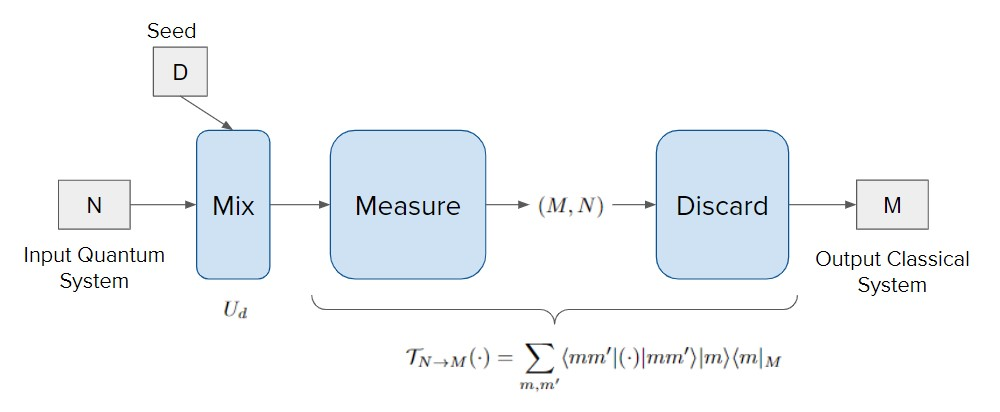
\includegraphics[scale=0.6]{Images/QC_extractor_definition.jpg}
    \caption{Quantum-to-Classical Extractor}
    \label{fig:qc_extractor}
\end{figure}

\subsection{Examples of QC-extractors}
 Two-independent hashing, also known as universal hashing, is one of the most important extractor constructions. We discussed this briefly in \autoref{sec:c_ext}. Basically, it includes selecting two hash functions from a family of hash functions such that it guarantees that the hash codes of both the designated keys are independent random variables \cite{impagliazzo1989pseudo}. In this article, we focus on the theory of unitary $2$-design, which can be seen as the quantum generalization of two-independent hash functions. 


There are many known efficient constructors of unitary $2$-designs [\cite{grossunitary}, \cite{dankert2design}], and in an $n$-qubit space, such unitaries can be computed with circuits of size $O(n^2)$. The following is immediate using a general decoupling result from \cite{dupuisdecoupling,oneshotdecoupling}.

\begin{corollary}
    Let $A = A_{1} \otimes A_{2}$ with $n = \log |A|$. For all $k \in [-n, n]$ and all $\eps > 0$, a unitary $2$-design $\set{U_1, ...., U_L}$ on $A$ is a $(k, \eps)$-QC-extractor with output size 
    $$\log |A_1| = \min{(n, n+k-2\log (1/\eps))}.$$
\end{corollary}
Similar results as above also hold true for "almost" $2$-design unitaries [\cite{osxehrtomamichel}, \cite{oszehrthesis}]. Now, by choosing a reasonably small $L$, making a set of random unitaries, with the seed size of the same order as the output size of the extractor, defines a QC-extractor with high probability. 




\begin{theorem}
    Let $A = A_{1} \otimes A_{2}$ with $n = \log |A|$ and let $\calT_{A \to A_{1}}: \calL(A) \to \calL(A_{2})$ the measurement map defined in \eqref{eq:measurement_map}. Let $\eps > 0$ and $c$ be a sufficiently large constant, and suppose that 
    \begin{align*}
        \log |A_{1}| 
        &\le n + k - 4 \log (1 / \eps) - c \quad \text{and} \quad 
        \log L 
        \geq \log |A_{1}| + \log n + 4 \log (1 / \eps) + c. 
    \end{align*}
    Then, choosing $\{U_{1}, \dots, U_{L}\}$ independently according to the Haar measure \cite{davis1955note} defines a $(k,\varepsilon)$-QC-extractor with high probability.
\end{theorem}

\subsection{Bitwise QC-extractor}
In this section, we discuss constructing simpler unitaries to define a QC-extractor. The construction is composed of unitaries $V$ acting on single qubits followed by permutations $P$ of the computational basis elements. Because the measurement $\calT$ and the permutations $P$ are commutative in nature, we first apply $V$, measure in the computational basis, and then finally apply the permutation  to the classical outcome of the measurement. Unitaries acting on single qubits is frequently a desired attribute for the design of cryptographic protocols, in addition to computational efficiency.

We consider a value $d \geq 2$ as a prime power so that there exists a complete set of mutually unbiased bases in dimension $d$. This set of bases can be represented by a set of unitary transformations given as $\set{V_0, V_1,..., V_d}$ which maps the mutually unbiased bases to some standard basis. The following example, we represent the unitary transformations when we take a full set of mutually unbiased bases in dimension $2$:
\begin{equation*}
    V_0 = 
    \begin{pmatrix}
    1 & 0 \\
    0 & 1 \\
    \end{pmatrix}
    \hspace{1cm}
    V_1 = \frac{1}{\sqrt{2}}
    \begin{pmatrix}
    1 & 1 \\
    1 & -1 \\
    \end{pmatrix}
    \hspace{1cm}
    V_2 = \frac{1}{\sqrt{2}} 
    \begin{pmatrix}
    1 & i \\
    i & -1 \\
    \end{pmatrix}
\end{equation*}

We now define the set $\calV_{d,n}$ of unitary transformations on n qubits as follows:
$$\calV_{d, n} := \set{V = V_{u_1} \otimes ... \otimes V_{u_n} | u_i \in \set{0, 1,..., d}}$$

\begin{theorem}
\label{theorem:bitwiseqc}
    Let $A = A_{1} \otimes A_{2}$ with $|A| = d^{n}$, $|A_{1}| = d^{\xi n}$, $|A_{2}| = d^{(1 - \xi) n}$ and $d$ a prime power. Then, for $\delta \ge 0$ and $\delta' > 0$,
    \begin{multline}
        \frac{1}{|\calP|} \frac{1}{(d + 1)^{n}} 
        \sum_{P \in \calP} \sum_{V \in \calV_{d, n}} 
        \left\|\calT_{A \to A_{1}} \left(P V \rho_{A E} (P V)^{\dagger}\right) - \frac{\I}{|A_{1}|} \otimes \rho_{E}\right\|_{1} \notag \\
        \le \sqrt{2^{(1 - \log(d + 1) + \xi \log d) n} (1 + 2^{- \Hmin^{\delta}(A | E)_{\rho} + z})} 
        + 2 (\delta + \delta'), 
    \end{multline}
    where $\calV_{d, n}$ is defined as above, $\calP$ is a family of pair-wise independent permutation matrices, and 
    \begin{align*}
        z = \log\left(\frac{2}{\delta'^{2}} + \frac{1}{1 - \delta}\right). 
    \end{align*}
    In particular, the set $\{P V: P \in \calP, V \in \calV_{d, n}\}$ is a $(k, \eps)$-QC-extractor provided
    \begin{align*}
        \log |A_{1}| 
        \le (\log(d + 1) - 1) n + \min\{0, k\} 
        - 4 \log(1 / \eps) - 7
    \end{align*}
    and the number of unitaries is $L = (d + 1)^{n} d^{n} (d^{n} - 1)$. 
\end{theorem}

\subsection{Full set of mutually unbiased bases (MUB)}

We saw that QC-extractors are defined by unitary 2-designs. It is reasonable to anticipate that we can create smaller and simpler sets of unitaries if we are simply interested in extracting random classical bits because unitary 2-designs also define QQ-extractors. Here, we build more basic sets of unitaries that define a QC-extractor, using a family of pair-wise independent permutations and a complete set of mutually unbiased bases.

\begin{definition}\normalfont{\textbf{(MUB)}} A \emph{mutually unbiased basis} is defined as the set of unitaries $\set{U_{1}, \dots, U_{L}}$ acting on $A$ such that a state described by a vector $U_{i}^{\dagger} \ket{a}$ of the basis $i$ gives a uniformly distributed outcome when measured in basis $j$ for $i \neq j$. There can be at most $|A| + 1$ mutually unbiased bases for $A$.  
\end{definition} 
\begin{definition}
    A family $\calP$ of of permutations of a set $X$ is called \emph{pair-wise independent} if for all $x_{1} \neq x_{2}$ and $y_{1} \neq y_{2}$, we have \[\Pr[\pi(x_{1}) = y_{1} \hbox{ and } \pi(x_{2}) = y_{2}] = \frac{1}{|X| (|X| - 1)},\]
for any $\pi$ uniformly distributed over $\calP$. 
\end{definition}

Observe that if $X$ is a field (so that $|X|$ is a prime power), the family 
\begin{align*}
    \calP = \{x \mapsto ax + b: x \in X^{*}, b \in X\}
\end{align*}
is pair-wise independent. Observing permutations of the basis elements of a Hilbert space $A$ as a unitary transformation on $A$, we have the following result.

\begin{theorem}
    Let $A = A_{1} \otimes A_{2}$ with $n = \log |A|$, where $|A|$ is a prime power. If $\{U_{1}, \dots, U_{|A| + 1}\}$ defines a full set of mutually unbiased bases, then for $\delta \ge 0$ we have
    \begin{multline}
        \frac{1}{|\calP|} \frac{1}{|A| + 1} 
        \sum_{P \in \calP} \!\!\sum_{i = 1}^{|A| + 1} 
        \left\|\calT_{A \to A_{1}} \left(P U_{i} \rho_{A E} (P U_{i})^{\dagger}\right) - \frac{\I_{A_{1}}}{|A_{1}|} \otimes \rho_{E}\right\|_{1} \notag
       \!\!\leq \sqrt{\frac{|A_1|2^{-H_{\min}(A|E)_{\rho}}}{|A_1|+1} } + 2\delta, 
    \end{multline}
    where $\calP$ is a set of pair-wise independent permutation matrices. In particular, the set $\set{P U_i: P \in \calP, i\in [|A|+1]}$ defines a $(k,\varepsilon)$-QC-extractor provided 
    \[\log|A_1| \leq n+k-2\log(1/\varepsilon),\]
    and the number of unitaries is 
    \[L = (|A|+1)\calP = (|A|+1)|A|(|A|-1).\]
\end{theorem}

The proofs of the above theorems require an understanding of concepts such as one-shot decoupling, permutation extractors, and advanced mathematical tools from linear algebra. Thus, due to page limit restrictions, for proof of the above theorems related to the construction of QC-extractors, we refer the reader to \cite{Berta_2014,berta2013quantum}.

We summarize all the results about QC-extractors in \autoref{table:summary} in the discussion section, i.e., \autoref{sec:discussion}.
\section{Applications}
In this section, we discuss the application of QC-extraction to achieve the performance of cryptographic models such as noisy storage models. We will mainly focus on two applications of QC-extractors. First, QC-extractor gives rise to entropic uncertainty relations with quantum side information, and second noisy storage model; in other words, any two-party cryptographic protocol can be implemented securely as long as the adversary’s storage device has sufficiently low quantum capacity.  

\subsection{Entropic uncertainty relations with quantum side information}
% \%\%\% \textcolor{red}{This paragraph gives ideas about uncertainty principle of physics.}
The uncertainty principle is one of the fundamental theories of quantum mechanics. 
Uncertainty relations, originally proposed by Heisenberg $\Delta x \Delta p \geq \frac{h}{4\pi}$, is one of the most prominent examples that show how quantum mechanics differs from the classical world. Perhaps, the best known in the form given by Robertson \cite{robertson1929uncertainty}, who extended Heisenberg's result to two arbitrary observables \footnote{In quantum physics, an observable is a physical quantity that can be measured, for example, position and momentum.} $A$ and $B$. Uncertainty relation states that if we prepare many copies of the state $\ket{\psi}$, and measure each copy individually using either observable $A$ or $B$, we have 
\[\Delta A \Delta B \geq \frac{1}{2} |\bra{\psi}[A,B]\ket{\psi}|\]
where $\Delta X = \sqrt{\bra{\psi}X^2\ket{\psi} - \bra{\psi}X\ket{\psi} }$ for $X = A, B$ is the standard deviation resulting from measuring $\ket{\psi}$ with observable $X$. This means that there is no way to simultaneously specify definite values of non-commuting\footnote{Two observables $A$ and $B$ are said to be commuting if $AB = BA$, thus, commutator $[A,B] = 0$,  where $ [A,B] = AB-BA$.} observables with great precision. 

% section IV of paper

Entropic uncertainty relations provide a contemporary way to express the notion of uncertainty in quantum mechanics. It has interesting applications in quantum cryptography, the entropic uncertainty relations allow to provide the security proof of cryptographic protocols.  Briefly, it provides a subtle interplay between uncertainty and entanglement.  We consider a bipartite guessing game, which consist of Alice and Eve, to understand the  entropic uncertainty relations. Entropic uncertainty relation allows us if Eve can or cannot predict the outcomes of two non-commuting measurements performed on Alice’s state.

% section 3.4 of https://ocw.tudelft.nl/wp-content/uploads/LN_Week3.pdf

Assume Eve only has classical memory, i.e., she might make measurements on the qubits during the transmission, but she cannot keep any entanglement with herself. This is equivalent to Eve preparing Alice’s qubits herself. We now define the \textit{guessing game} below:

\begin{tcolorbox}
    {\bf Guessing Game:}
    \begin{enumerate}
        \item {\bf Eve:} Prepares a qubit $\rho_{A}$ and sends it to Alice
        \item {\bf Alice:} Chooses a random bit $\Theta \in \{0, 1\}$
        \item {\bf Alice:} If $\Theta = 0$, then Alice measures $\rho_{A}$ in the computational basis,  i.e., $\set{\ket{0},\ket{1}}$; otherwise, she measures $\rho_{A}$ in the Hadamard basis,  i.e., $\set{\ket{+},\ket{-}}$
        \item {\bf Alice:} Records the measurement outcome $X \in \{0, 1\}$
        \item {\bf Alice:} Announces $\Theta$
        \item {\bf Eve:} Wins if she correctly guesses $X$
    \end{enumerate}
\end{tcolorbox}
\begin{figure}
    \centering
    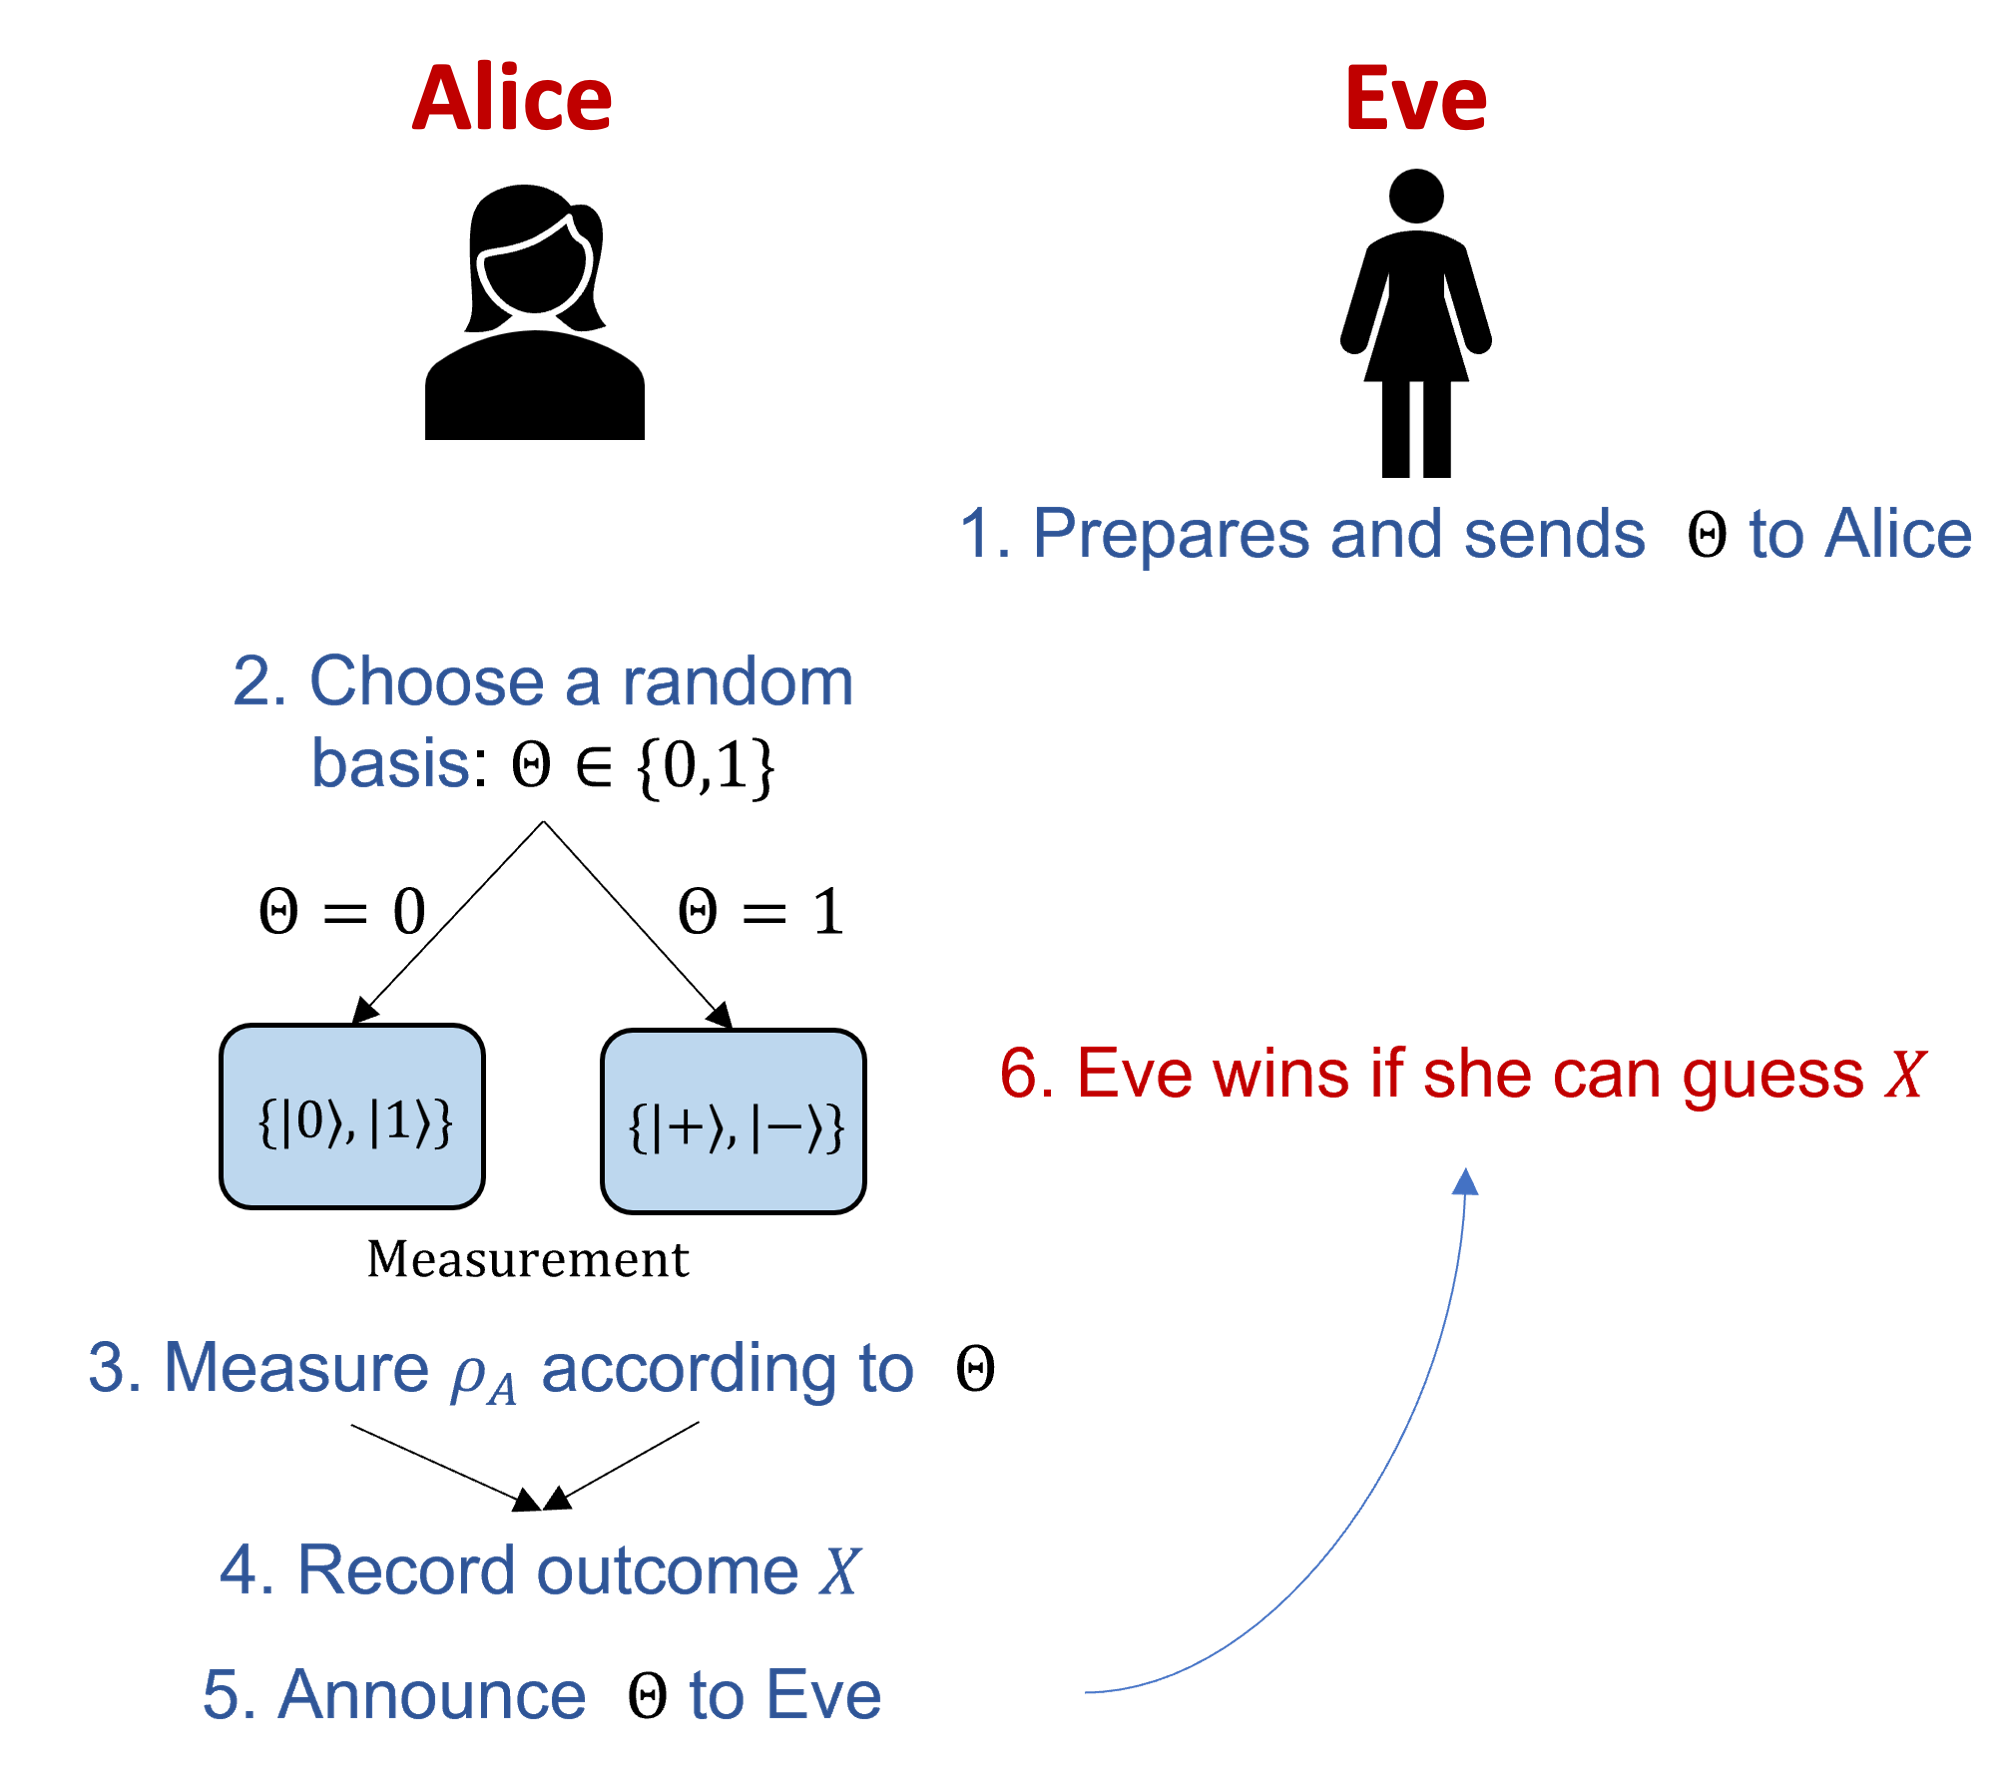
\includegraphics[scale=0.5]{Images/uncertainty.png}
    \caption{The bipartite guessing game between Alice and Eve.}
    \label{fig:uncertainty}
\end{figure}
\autoref{fig:uncertainty} summarizes the guessing game defined above. The objective is to make sure that Eve cannot fully predict Alice’s measurement outcome. Consider the following example, where the joint state between Alice and Eve is 
\begin{align*}
    \rho_{A E} 
    &= \ket{0} \bra{0}_{A} \otimes \rho_{E},
\end{align*}
where Alice measures system $A$ in either the computational or the Hadamard basis to obtain the secret key. 
To see why this captures the essence of the uncertainty principle, note that if the measurements are non-commuting, then there exists no state $\rho_{A}$ that Eve can prepare, which would allow her to guess the outcome for both choices of measurements with certainty. Uncertainty can be understand as  a bound on the average probability that Eve correctly guesses $X$:
\begin{align*}
    \Pr[X \mid \Theta] 
    &= \Pr[\Theta = 0] \cdot \Pr[X \mid \Theta = 0] + 
    \Pr[\Theta = 1] \cdot \Pr[X \mid \Theta = 1] \\
    &= \frac{1}{2} [\Pr[X \mid \Theta = 0] + \Pr[X \mid \Theta = 1]\le \epsilon,
\end{align*}
where the second equality holds if Alice chooses her measurement basis $\Theta$ at random, i.e. with uniform probability $1 / 2$ for each option. In the case where Eve holds no additional information except for the basis where Alice has performed the measurement, it can be shown that $\epsilon < 1$. To understand this, suppose Eve always aims to correctly guess $X$ regardless of whether $\Theta = 0$ or $\Theta = 1$. Then she requires $\Pr[X \mid \Theta = 0] = 1$, i.e. she should prepare a state that will always produce a deterministic outcome when Alice measures in the computational basis. In order for this to happen, Eve can send the state $\ket{0} \bra{0}_{A}$, where Alice, upon measuring in the computational basis, will always produce $X = 0$. However, if Eve has used the strategy of preparing $\ket{0} \bra{0}_{A}$ and Alice measures in the Hadamard basis, then
\begin{align*}
    \Pr[X \mid \Theta = 1] 
    &= \max\{\Pr[X = 0 \mid \Theta = 1], \Pr[X = 1 \mid \Theta = 1] \\
    &= \max\{\Tr[\ket{+} \bra{+} \ket{0} \bra{0}], \Tr[\ket{-} \bra{-} \ket{0} \bra{0}]\}= \frac{1}{2}. 
\end{align*}
Thus, if Eve uses this strategy of preparing $\rho_{A} = \ket{0} \bra{0}_{A}$ in order to guess Alice’s outcome $X$, then whenever $\Theta = 1$, this corresponds only to a random guess. So, in this protocol, since Eve does not know beforehand what basis Alice will choose to measure in, she has to prepare a state that will maximize her guessing probability in both cases of Alice measuring in the standard basis, and also the Hadamard basis. The above example shows that this guessing probability can never be equal to $1$.

Note that in order for Eve to maximize the guessing probability $\Pr[X \mid \Theta]$ over $\rho_{A}$, without loss of generality, we consider the outcome to be $X = 0$,
\begin{align*}
    \Pr[X \mid \Theta] 
    &= \frac{1}{2} (\Tr[\rho_{A} \ket{0} \bra{0}] + \Tr[\rho_{A} \ket{+} \bra{+}])= \frac{1}{2} \Tr[\rho_{A} (\ket{0} \bra{0} + \ket{+} \bra{+})]
\end{align*}
then she has to prepare $\rho_{A}$ in the pure state corresponding to the eigenvector of $\ket{0} \bra{0} + \ket{+} \bra{+}$ with the largest eigenvalue, which is $\lambda_{\max} 
    = 1 + {1/\sqrt{2}}.$
% \begin{align*}
%     \lambda_{\max} 
%     &= 1 + \frac{1}{\sqrt{2}}.
% \end{align*}
Therefore,
\begin{align*}
    \Pr[X |\Theta] 
    &= \frac{1}{2} + \frac{1}{2 \sqrt{2}} 
    < 1.
\end{align*}

To calculate Eve's guessing probability, we write a quantum state in the following form \cite{wilde2013quantum,nielsen2002quantum}:
\begin{align*}
    \rho_{A} 
    &= \frac{1}{2} (\I + v_{x} X + v_{y} Y + v_{z} Z)
\end{align*}
for a vector $v = (v_{x}, v_{y}, v_{z})$. Then,
\begin{align*}
    &\Tr[\rho_{A} \ket{0} \bra{0}] 
    = \frac{1}{2} (1 + v_{z}), 
    &\Tr[\rho_{A} \ket{1} \bra{1}] 
    = \frac{1}{2} (1 - v_{z}), \\
    &\Tr[\rho_{A} \ket{+} \bra{+}] 
    = \frac{1}{2} (1 + v_{x}), 
    &\Tr[\rho_{A} \ket{-} \bra{-}] 
    = \frac{1}{2} (1 - v_{x}). 
\end{align*}
\begin{align*}
    \text{Also, } \Pr[X \mid \Theta] 
    &= \frac{1}{2} \max\{\Tr[\rho_{A} \ket{0} \bra{0}], \Tr[\rho_{A} \ket{1} \bra{1}]\} + 
    \frac{1}{2} \max\{\Tr[\rho_{A} \ket{+} \bra{+}], \Tr[\rho_{A} \ket{-} \bra{-}]\}
\end{align*}
maximized over all possible states $\rho_{A}$. Since the maximizations of both expression are symmetric around $v_{z} = 0, v_{x} = 0$, respectively.  Consider only the case where $v_{z}, v_{x} \ge 0$. Thus, we get,
\begin{align*}
    \Pr[X \mid \Theta]_{\rho_{A}} 
    &= \frac{1}{2} \Tr[\rho_{A} (\ket{0} \bra{0} + \ket{+} \bra{+})] = \frac{1}{4} (2 + v_{x} + v_{z}), \qquad v_{x}^{2} + v_{z}^{2} \le 1.
\end{align*}
Note that the maximum occurs when $v_{x}^{2} + v_{z}^{2} = 1$. 
% Letting $v_{x} = \cos(t)$, $v_{z} = \sin(t)$ gives that
% \begin{align*}
%     \max_{t} \{\cos(t) + \sin(t)\}
% \end{align*}
% obtained for $\cos(t) = \sin(t) = 1 / \sqrt{2}$. 
Therefore, by the change of variable as  $v_{x} = \cos(t)$, $v_{z} = \sin(t)$, we get,  the probability of Eve winning the game is 
\begin{align*}
    \Pr[X \mid \Theta]_{\rho_{A}} 
    &= \frac{1}{2} + \frac{1}{2 \sqrt{2}} 
    \approx 0.85.
\end{align*}
In a more general scenario, Eve may even have classical information about $\rho_{A}$. Following the same steps as above, we can show that 
\begin{align*}
    \Pr[X | \Theta C]_{\rho_{AC}} 
    &= \frac{1}{2} + \frac{1}{2 \sqrt{2}} 
    \approx 0.85.
\end{align*}
Thus, the min-entropy $\Hmin(X \mid \Theta C) = - \log \Pr[X \mid \Theta C] \approx 0.22$. 

If we always allow Eve maximum information about everything, she may prepare a larger state $\rho_{AE}$,  i.e., Eve also holds the purification and send the $\rho_A$ to Alice.  Then one can show that if Eve can be entangled with Alice’s qubit, then she can guess perfectly.

Finally, if we want to keep $X$ secret from Eve, we need to use two aspects of quantum mechanics:
\begin{enumerate}
    \item Uncertainty: If Eve has no (or little) entanglement with Alice, then she cannot certainly predict the outcomes of two non-commuting measurements. So it is difficult to guess Alice’s measurement outcomes, i.e., $\Pr[X | E \Theta] < 1$, or equivalently, $\Hmin(X | E \Theta) > 0$.
    \item Entanglement: We need to ensure there exists some entanglement between Alice and Eve. For this, we can use the fact that entanglement is \textit{monogamous} \footnote{Please see the page on Wikipedia \href{https://en.wikipedia.org/wiki/Monogamy_of_entanglement}{Monogamy of entanglement}}, that is if we find a large amount of entanglement between Alice and Bob, then we know that Eve has very little entanglement with either Alice or Bob, and therefore the min-entropy should be large. Hence, Eve cannot guess the outcome of Alice, and entropic uncertainty ensures security!
\end{enumerate}

% https://ocw.tudelft.nl/course-lectures/3-4-1-uncertainty-principles-simple-version-bb84/
% table on page 17


Below, in \autoref{tab:lower_bounds}, we summarize the various methods used for constructing QC-extractions to achieve the uncertainty relations for the min-entropy \cite{berta2013quantum,Berta_2014}:

\begin{table}[h]
    \centering
    \begin{tabular}{|l|c|}
        \hline
         & Lower bounds for smooth conditional min-entropy $\Hmin$ \\
        \hline 
        Unitary $2$-design & $\log |A| + \Hmin^{\delta}(A | E)_{\rho} - \log\left(\frac{1}{(\varepsilon^{2} / 2 - 2 \delta)^{2}}\right)$ \\
        \hline
        Almost unitary $2$-design & $\log |A| + \Hmin^{\delta}(A | E)_{\rho} - \log\left(\frac{1}{(\varepsilon^{2} / 2 - 2 \delta)^{2}}\right) - \log(1 + \zeta)$ \\
        \hline
        All $|A| + 1$ MUBs & $\log(|A| + 1) + \Hmin^{\delta}(A | E)_{\rho} - \log\left(\frac{1}{(\varepsilon^{2} / 2 - 2 \delta)^{2}}\right)$ \\
        \hline
        Single qudit MUBs & $n (\log(d + 1) - 1) + \min\left\{0, \Hmin^{\delta}(A | E)_{\rho} - \log\left(\frac{2}{\delta'^{2}} + \frac{1}{1 - 2 \delta}\right)\right\}$ \\
        & \hfill $ - \log\left(\frac{1}{(\varepsilon^{2} / 2 - 2 \delta - \delta')^{2}}\right) - 1$\\
        \hline
    \end{tabular}
    \vspace{5pt}
    \caption{Entropic uncertainty relations with quantum side information for the smooth conditional min-entropy for approximation parameters $\varepsilon > 0$, $\zeta \ge 0$, $\delta \ge 0$, and $\delta' > 0$.}
    \label{tab:lower_bounds}
\end{table}

\subsection{Noisy-Storage Model}

Quantum computer benefits computing resources for those algorithms with computational assumptions, but a drawback is that the security can be broken retroactively. Most two-party protocols that have been executed to date will lose their security because the adversary can use the quantum computer to break the protocol. One way to solve this problem is to consider physical assumptions rather than computational assumptions. The most straightforward one is storage. 

In classical cryptography, physical assumptions are usually made as the \emph{bounded-storage model}, which assumes that the adversary can only store a certain number of classical bits. After introducing quantum communication, one now assumes that the adversary's quantum storage is limited to a certain number of qubits but no restriction on the classical bits. This is known as \emph{bounded-quantum-storage model}. More generally, one can also invoke the noisy storage model, where the quantum storage is not only bounded but also noisy in general \cite{tudelftQC}, to incorporate both the amount of storage and noise. \cite{Konig_2012} introduced the concept of a \emph{noisy-storage model}.

\begin{definition}\textbf{(Noisy Quantum Memory)}
Given a device whose input states are in some Hilbert space $\mathcal{H}_{in}$, a \emph{noisy quantum memory} is a state $\rho$ stored in the device decoheres over time. That is, the content of the memory after some time $t$ is a state $\mathcal{F}_t(\rho)$, where $\mathcal{F}_t : \mathcal{H}_{in} \rightarrow \mathcal{H}_{out}$ is a completely positive trace-preserving map corresponding to the noise in the memory.

Considering the security, the intuition is that security is possible as long as the amount of information that the adversary can store in his memory device is limited. Therefore, the central assumption of the model is that during waiting times $\delta t$ introduced into the protocol, the adversary can only store quantum information using a limited and unreliable quantum memory device. In particular, the adversary can store an unlimited amount of classical information while also doing any operation at the moment. That means he is able to use any encoding and decoding operations before and after using his memory device. Notice that the input spaces can be in the form of $\mathcal{H}_{in} = (\C^d)^{\otimes N}$ and channels $\mathcal{F} = \mathcal{N}^{\otimes N}$ with $\mathcal{N}: \mathcal{H}_{in} \rightarrow \mathcal{H}_{out}$.

To analyze the security of a noisy-storage model, we first introduce a technique called \emph{weak string ensure}.

\begin{definition}\textbf{(Weak String Erasure)}
In a two-party secure computation, \emph{weak string erasure} is a primitive that provides Alice with a random bit string $X^n \in \{0,1\}^n$ and Bob with a randomly chosen substring $X_{\mathcal{I} = (X_{i_1}, X_{i_2}, \dots, X_{i_r})}$ together with index set $\mathcal{I} = \{i_1, i_2, \dots, i_r\}$ specifying the location of these bits \cite{Konig_2012}.
\end{definition}

The motivation behind the primitive weak string erasure was to create a basic quantum protocol that builds up classical correlations between Alice and Bob which are later used to implement more interesting cryptographic primitives. We can construct a very simple protocol for weak string erasure and prove its security using a bitwise QC-randomness extractor.

The protocol is basically the same as the one provided in \cite{Konig_2012}, but in our case, instead of using only 2 MUBs per qubit, there will be 3. The procedure is as follows: 
\begin{tcolorbox}
\textbf{Protocol Weak String Erasure (WSE):} 
\newline
\textbf{Output: }$x^n \in \{0,1\}^n$ \textbf{to Alice,} $(\mathcal{I, |z|^{\mathcal{I}}}) \in 2^{[n]} \times \{0,1\}^{\mathcal{I}}$ \textbf{to Bob.}
\\ \hspace*{\fill} \\
\hspace*{0.5cm} \textbf{1. Alice:} Creates $n$ EPR-pairs $\Phi$, and sends half of each pair to Bob.
\newline
\hspace*{0.5cm} \textbf{2. Alice:} Chooses a bases-specifying string $\theta^n \in_R \{0,1,2\}^n$ uniformly at random. 
\newline
\hspace*{1cm} For all $i$, she measures the $i$-th qubit in the basis $\theta_i$ to obtain outcome $x_i$.
\newline
\hspace*{0.5cm} \textbf{3. Bob: } Chooses a basis string $\tilde{\theta}_i \in_R \{0,1,2\}^n$ uniformly at random. When 
\newline
\hspace*{1cm} receiving the $i$-th qubit, Bob measures it in the basis of $\tilde{\theta}^n$ to obtain outcome $\tilde{x}_i$.
\\ \hspace*{\fill} \\
Both parties wait time $\Delta t$. 
\\ \hspace*{\fill} \\
\hspace*{0.5cm} \textbf{4. Alice: } Sends the basis information $\theta^n$ to Bob and outputs $x^n$.
\newline
\hspace*{0.5cm} \textbf{5. Bob: } Computes $\mathcal{I} = \{i \in [n] | \theta_i = \tilde{\theta}_i\}$, and outputs $(\mathcal{I, |z|^{\mathcal{I}}}) := (\mathcal{I}, \tilde{x}_{\mathcal{I}})$.
\end{tcolorbox}

The proof of the correctness of the protocol and in regards to a dishonest Alice can be found in \cite{Konig_2012}. To prove the security against a dishonest Bob, we first consider the general form that any attack on Bob takes in the \autoref{fig:nsm2}.

\begin{figure}[!htb]
    \centering
    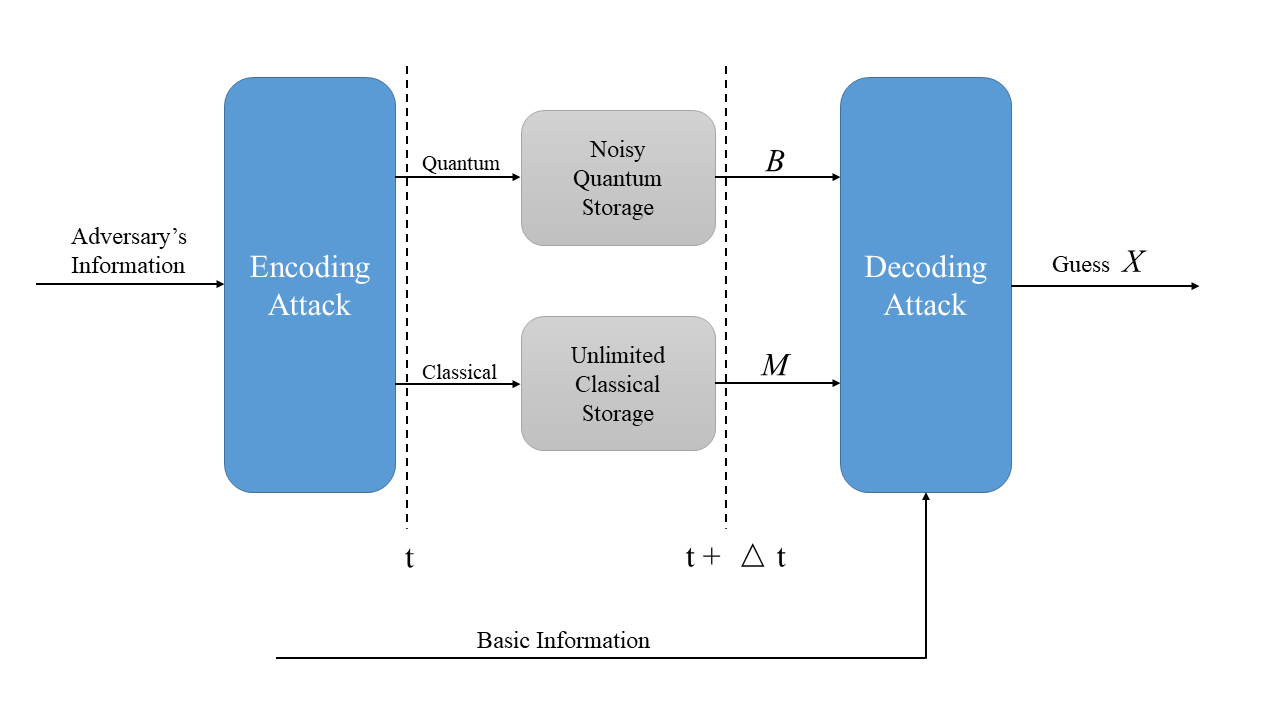
\includegraphics[scale=0.37]{Images/NSM2.png}
    \caption{Any attack of dishonest Bob is described by an encoding attack $E$ and a ‘guessing’ attack.}
     \label{fig:nsm2}
\end{figure}
% \newline
% \newline

Note that the noisy-storage model only assumes that Bob has to use his storage device during waiting times $\delta t$, which means when attacking the protocol above, he can store the incoming qubits perfectly until $n$ qubits arrive. Let $\mathcal{Q}$ denote Bob’s quantum register containing all $n$ qubits. Since there is no communication between Alice and Bob during the transmission of these n qubits, we can assume that Bob first waits for all n qubits to arrive before mounting any form of attack. Besides, as any operation in quantum theory is a quantum channel, Bob’s attack can be described by a quantum channel $\mathcal{E}: \mathcal{S}_{\leq}(\mathcal{Q}) \rightarrow \mathcal{S}_{\leq}(\mathcal{H}_{in} \otimes M)$, where this map takes $\mathcal{Q}$ to some quantum state on the input of Bob's storage device, $\mathcal{H}_{in}$, and $M$, some arbitrarily large amount of classical information. For example, $\mathcal{E}$ could be an encoding into an error-correcting code. 

Then, by the assumption of the noisy-storage model, Bob’s quantum memory is then affected by noise $\mathcal{F}: \mathcal{S}_{\leq}(\mathcal{H}_{in}) \rightarrow \mathcal{S}_{\leq}(\mathcal{H}_{out})$. After the waiting time, the joint state held by Alice and Bob in the purified version of the protocol (i.e., before Alice measures) is thus of the form

$$\rho_{ABM} = \mathcal{I}_A \otimes [(\mathcal{F} \otimes \mathcal{I}_M) \circ \mathcal{E}](\Phi^{\otimes n})$$

where $\Phi$ is an EPR-pair. And after the waiting time, Bob can perform any form of quantum operation to try and recover information from the storage device. Note that, in principle, Bob’s goal is to recover $X$ alone, for which he could potentially use his basis information $\Theta$. In fact, we can ignore the basis information in the analysis. That is, we only need to analyze decoding maps $\mathcal{D}: \mathcal{S}_{\leq}(\mathcal{H}_{in} \otimes M) \rightarrow \mathcal{S}_{\leq}(\mathcal{Q})$ trying to recover the initial entanglement between Alice and Bob.

After implementing the task of `Weak String Erasure' as above, we consider the usage of bitwise QC-extrators as linking security to the entanglement fidelity (quantum capacity) of the noisy quantum storage. Earlier, we came across the fact that one of the desirable properties of a bitwise QC-extrator is that, in addition to its computational efficiency, we observe that the unitaries act on single qubits. So, by changing the encoding from a qubit scheme to a qubit six-state scheme, we use the bitwise QC-extrator, defined in Theorem \ref{theorem:bitwiseqc}. This gives us a strong converse classical capacity replaced by the strong converse quantum capacity. This then extends the parameter regime where the security of all existing protocols can be proven.  Even though there is in general, no closed expression for the strong converse quantum capacity, we can calculate security rates by means of the entanglement cost of quantum channels, which is an upper bound on the strong converse quantum capacity. As a brief overview, the entanglement cost of a quantum channel is the minimal rate at which entanglement (between sender and receiver) is needed in order to simulate many copies of a quantum channel in the presence of free classical communication.
\end{definition}
\section{Discussion} \label{sec:discussion}
%As you can see, this problem is very similar to
%privacy amplification, but without the added complication of Alice having to coordinate with Bob!

In this report, we introduced the concept of a randomness extractor. We discussed classical randomness extractors and provided examples and applications, namely, 2-universal extractors. We further discussed the concept of quantum-to-classical randomness extractors. We showed that for a QC-extractor to distill randomness from a quantum state $\rho_{AE}$, the relevant quantity to bound is the conditional min-entropy $\Hmin(A | E)_{\rho}$. This is in formal analogy with classical-to-classical extractors, in which case the relevant quantity is $\Hmin(X | E)_{\rho}$.

We showed various properties of QC-extractors and gave several examples for QC-extractors. We compare our results about QC-extractors with CC-extractors in \autoref{table:summary}.

\begin{table}[h]
    \centering
    \begin{tabular}{|l|l|c|c|}
    \hline
        & & CC-extractors & QC-extractors \\\hline 
        Seed & Lower bound & $\log(n - k) + 2 \log(1 / \varepsilon)$ & $\log(1 / \varepsilon)$ \\
        & Upper bounds & $\log(n - k) + 2 \log(1 / \varepsilon)$ (NE) & $m + \log n + 4 \log(1 / \varepsilon)$ \\
        & & $c \log(n / \varepsilon)$ & $3 n$ \\\hline 
        Output & Upper bound & $k - 2 \log(1 / \varepsilon)$ & $n + \Hmin^{\sqrt{\varepsilon}}(A | E)$ \\
        & Lower bound & $k - 2 \log(1 / \varepsilon)$ & $n + k - 2 \log(1 / \varepsilon)$ \\\hline
    \end{tabular}
    \vspace{5pt}
    \caption{Bounds on the seed size and output size in terms of (qu)bits for different kinds of $(k, \varepsilon)$-randomness extractors. Here, n refers to the number of input (qu)bits, $m$ the number of output (qu)bits, and $k$ the min-entropy of the input $\Hmin(A | E)$.}
    \label{table:summary}
\end{table}

There is an extensive difference between the upper and lower bounds for the seed size of QC-extractors. We were only able to show the existence of QC-extractors with seed length roughly the output size $m$, but we believe that it should be possible to find QC-extractors with much smaller seeds, say $O({\rm polylog}(n))$ bits long, where $n$ is the input size. However, entirely different techniques might be needed to address this question.

We showed that every QC-extractor gives rise to entropic uncertainty relations with quantum side information for the Von Neumann (Shannon) entropy and the min-entropy. Here the seed size translates into the number of measurements in the uncertainty relation. Since it is, in general difficult to obtain uncertainty relations for a small set of measurements (except for the special case of two), finding QC-extractors with a small seed size is also worth pursuing from the point of view of uncertainty relations.

We used the bitwise QC-extractor from \autoref{sec:qc_ext} to show that the security in the noisy storage model can be related to the strong converse rate of the quantum storage, a problem that attracted quite some attention over the last few years. Here one can also see the usefulness of bitwise QC-extractors for quantum cryptography. Indeed, any bitwise QC-extractor would yield a protocol for weak string erasure. Bitwise measurements have a very simple structure and hence are implementable with current technology. In that respect, it would be interesting to see if a similar QC-extractor can also be proven for only two (complementary) measurements per qubit. This would give a protocol for weak string erasure. It is expected that QC-extractors will have many more applications in quantum cryptography, e.g., quantum key distribution and privacy amplification.

We encourage the reader to go through the following video, which provides a brief overview of the topic:
\href{https://tinyurl.com/eecs572projectvideo}{Quantum-to-Classical Randomness Extractor\footnote{https://tinyurl.com/eecs572projectvideo}.}
% \section{[Points to be included in the final report]}
% \begin{itemize}
%      \item We will discuss another construction of QC extractor, namely, full set of mutually unbiased bases (MUBs), alongwith the proof.
%     \item We will extensively discuss two applications of QC extractors, the entropic uncertainty relation and noisy storage model.
%     \item Proof of Theorem 4.4 and Theorem 4.5.
%     \item We will briefly discuss few explicit construction of CC-randomness extractor.
%     \item We will add more definitions in the preliminaries section as required, based on the addition of further contents.
%     % , for example quantum side information (highlighted in red in Section 4).
%     % \item We will briefly discuss about the Quantum-to-Quantum randomness extractor. 
% \end{itemize}
%%%%%%%%%%%%%%%%%%%%%%%%%%%%%%%%%%%%%%%%%%%%%%%%
\begin{comment}
\section{Submission of papers to NeurIPS 2021}

Please read the instructions below carefully and follow them faithfully.

\subsection{Style}

Papers to be submitted to NeurIPS 2021 must be prepared according to the
instructions presented here. Papers may only be up to {\bf nine} pages long,
including figures. Additional pages \emph{containing only acknowledgments and
references} are allowed. Papers that exceed the page limit will not be
reviewed, or in any other way considered for presentation at the conference.

The margins in 2021 are the same as those in 2007, which allow for $\sim$$15\%$
more words in the paper compared to earlier years.

Authors are required to use the NeurIPS \LaTeX{} style files obtainable at the
NeurIPS website as indicated below. Please make sure you use the current files
and not previous versions. Tweaking the style files may be grounds for
rejection.

\subsection{Retrieval of style files}

The style files for NeurIPS and other conference information are available on
the World Wide Web at
\begin{center}
  \url{http://www.neurips.cc/}
\end{center}
The file \verb+neurips_2021.pdf+ contains these instructions and illustrates the
various formatting requirements your NeurIPS paper must satisfy.

The only supported style file for NeurIPS 2021 is \verb+neurips_2021.sty+,
rewritten for \LaTeXe{}.  \textbf{Previous style files for \LaTeX{} 2.09,
  Microsoft Word, and RTF are no longer supported!}

The \LaTeX{} style file contains three optional arguments: \verb+final+, which
creates a camera-ready copy, \verb+preprint+, which creates a preprint for
submission to, e.g., arXiv, and \verb+nonatbib+, which will not load the
\verb+natbib+ package for you in case of package clash.

\paragraph{Preprint option}
If you wish to post a preprint of your work online, e.g., on arXiv, using the
NeurIPS style, please use the \verb+preprint+ option. This will create a
nonanonymized version of your work with the text ``Preprint. Work in progress.''
in the footer. This version may be distributed as you see fit. Please \textbf{do
  not} use the \verb+final+ option, which should \textbf{only} be used for
papers accepted to NeurIPS.

At submission time, please omit the \verb+final+ and \verb+preprint+
options. This will anonymize your submission and add line numbers to aid
review. Please do \emph{not} refer to these line numbers in your paper as they
will be removed during generation of camera-ready copies.

The file \verb+neurips_2021.tex+ may be used as a ``shell'' for writing your
paper. All you have to do is replace the author, title, abstract, and text of
the paper with your own.

The formatting instructions contained in these style files are summarized in
Sections \ref{gen_inst}, \ref{headings}, and \ref{others} below.

\section{General formatting instructions}
\label{gen_inst}

The text must be confined within a rectangle 5.5~inches (33~picas) wide and
9~inches (54~picas) long. The left margin is 1.5~inch (9~picas).  Use 10~point
type with a vertical spacing (leading) of 11~points.  Times New Roman is the
preferred typeface throughout, and will be selected for you by default.
Paragraphs are separated by \nicefrac{1}{2}~line space (5.5 points), with no
indentation.

The paper title should be 17~point, initial caps/lower case, bold, entered
between two horizontal rules. The top rule should be 4~points thick and the
bottom rule should be 1~point thick. Allow \nicefrac{1}{4}~inch space above and
below the title to rules. All pages should start at 1~inch (6~picas) from the
top of the page.

For the final version, authors' names are set in boldface, and each name is
centered above the corresponding address. The lead author's name is to be listed
first (left-most), and the co-authors' names (if different address) are set to
follow. If there is only one co-author, list both author and co-author side by
side.

Please pay special attention to the instructions in Section \ref{others}
regarding figures, tables, acknowledgments, and references.

\section{Headings: first level}
\label{headings}

All headings should be lower case (except for first word and proper nouns),
flush left, and bold.

First-level headings should be in 12-point type.

\subsection{Headings: second level}

Second-level headings should be in 10-point type.

\subsubsection{Headings: third level}

Third-level headings should be in 10-point type.

\paragraph{Paragraphs}

There is also a \verb+\paragraph+ command available, which sets the heading in
bold, flush left, and inline with the text, with the heading followed by 1\,em
of space.

\section{Citations, figures, tables, references}
\label{others}

These instructions apply to everyone.

\subsection{Citations within the text}

The \verb+natbib+ package will be loaded for you by default.  Citations may be
author/year or numeric, as long as you maintain internal consistency.  As to the
format of the references themselves, any style is acceptable as long as it is
used consistently.

The documentation for \verb+natbib+ may be found at
\begin{center}
  \url{http://mirrors.ctan.org/macros/latex/contrib/natbib/natnotes.pdf}
\end{center}
Of note is the command \verb+\citet+, which produces citations appropriate for
use in inline text.  For example,
\begin{verbatim}
   \citet{hasselmo} investigated\dots
\end{verbatim}
produces
\begin{quote}
  Hasselmo, et al.\ (1995) investigated\dots
\end{quote}

If you wish to load the \verb+natbib+ package with options, you may add the
following before loading the \verb+neurips_2021+ package:
\begin{verbatim}
   \PassOptionsToPackage{options}{natbib}
\end{verbatim}

If \verb+natbib+ clashes with another package you load, you can add the optional
argument \verb+nonatbib+ when loading the style file:
\begin{verbatim}
   \usepackage[nonatbib]{neurips_2021}
\end{verbatim}

As submission is double blind, refer to your own published work in the third
person. That is, use ``In the previous work of Jones et al.\ [4],'' not ``In our
previous work [4].'' If you cite your other papers that are not widely available
(e.g., a journal paper under review), use anonymous author names in the
citation, e.g., an author of the form ``A.\ Anonymous.''

\subsection{Footnotes}

Footnotes should be used sparingly.  If you do require a footnote, indicate
footnotes with a number\footnote{Sample of the first footnote.} in the
text. Place the footnotes at the bottom of the page on which they appear.
Precede the footnote with a horizontal rule of 2~inches (12~picas).

Note that footnotes are properly typeset \emph{after} punctuation
marks.\footnote{As in this example.}

\subsection{Figures}

\begin{figure}
  \centering
  \fbox{\rule[-.5cm]{0cm}{4cm} \rule[-.5cm]{4cm}{0cm}}
  \caption{Sample figure caption.}
\end{figure}

All artwork must be neat, clean, and legible. Lines should be dark enough for
purposes of reproduction. The figure number and caption always appear after the
figure. Place one line space before the figure caption and one line space after
the figure. The figure caption should be lower case (except for first word and
proper nouns); figures are numbered consecutively.

You may use color figures.  However, it is best for the figure captions and the
paper body to be legible if the paper is printed in either black/white or in
color.

\subsection{Tables}

All tables must be centered, neat, clean and legible.  The table number and
title always appear before the table.  See Table~\ref{sample-table}.

Place one line space before the table title, one line space after the
table title, and one line space after the table. The table title must
be lower case (except for first word and proper nouns); tables are
numbered consecutively.

Note that publication-quality tables \emph{do not contain vertical rules.} We
strongly suggest the use of the \verb+booktabs+ package, which allows for
typesetting high-quality, professional tables:
\begin{center}
  \url{https://www.ctan.org/pkg/booktabs}
\end{center}
This package was used to typeset Table~\ref{sample-table}.

\begin{table}
  \caption{Sample table title}
  \label{sample-table}
  \centering
  \begin{tabular}{lll}
    \toprule
    \multicolumn{2}{c}{Part}                   \\
    \cmidrule(r){1-2}
    Name     & Description     & Size ($\mu$m) \\
    \midrule
    Dendrite & Input terminal  & $\sim$100     \\
    Axon     & Output terminal & $\sim$10      \\
    Soma     & Cell body       & up to $10^6$  \\
    \bottomrule
  \end{tabular}
\end{table}

\section{Final instructions}

Do not change any aspects of the formatting parameters in the style files.  In
particular, do not modify the width or length of the rectangle the text should
fit into, and do not change font sizes (except perhaps in the
\textbf{References} section; see below). Please note that pages should be
numbered.

\section{Preparing PDF files}

Please prepare submission files with paper size ``US Letter,'' and not, for
example, ``A4.''

Fonts were the main cause of problems in the past years. Your PDF file must only
contain Type 1 or Embedded TrueType fonts. Here are a few instructions to
achieve this.

\begin{itemize}

\item You should directly generate PDF files using \verb+pdflatex+.

\item You can check which fonts a PDF files uses.  In Acrobat Reader, select the
  menu Files$>$Document Properties$>$Fonts and select Show All Fonts. You can
  also use the program \verb+pdffonts+ which comes with \verb+xpdf+ and is
  available out-of-the-box on most Linux machines.

\item The IEEE has recommendations for generating PDF files whose fonts are also
  acceptable for NeurIPS. Please see
  \url{http://www.emfield.org/icuwb2010/downloads/IEEE-PDF-SpecV32.pdf}

\item \verb+xfig+ "patterned" shapes are implemented with bitmap fonts.  Use
  "solid" shapes instead.

\item The \verb+\bbold+ package almost always uses bitmap fonts.  You should use
  the equivalent AMS Fonts:
\begin{verbatim}
   \usepackage{amsfonts}
\end{verbatim}
followed by, e.g., \verb+\mathbb{R}+, \verb+\mathbb{N}+, or \verb+\mathbb{C}+
for $\mathbb{R}$, $\mathbb{N}$ or $\mathbb{C}$.  You can also use the following
workaround for reals, natural and complex:
\begin{verbatim}
   \newcommand{\RR}{I\!\!R} %real numbers
   \newcommand{\Nat}{I\!\!N} %natural numbers
   \newcommand{\CC}{I\!\!\!\!C} %complex numbers
\end{verbatim}
Note that \verb+amsfonts+ is automatically loaded by the \verb+amssymb+ package.

\end{itemize}

If your file contains type 3 fonts or non embedded TrueType fonts, we will ask
you to fix it.

\subsection{Margins in \LaTeX{}}

Most of the margin problems come from figures positioned by hand using
\verb+\special+ or other commands. We suggest using the command
\verb+\includegraphics+ from the \verb+graphicx+ package. Always specify the
figure width as a multiple of the line width as in the example below:
\begin{verbatim}
   \usepackage[pdftex]{graphicx} ...
   \includegraphics[width=0.8\linewidth]{myfile.pdf}
\end{verbatim}
See Section 4.4 in the graphics bundle documentation
(\url{http://mirrors.ctan.org/macros/latex/required/graphics/grfguide.pdf})

A number of width problems arise when \LaTeX{} cannot properly hyphenate a
line. Please give LaTeX hyphenation hints using the \verb+\-+ command when
necessary.

\begin{ack}
Use unnumbered first level headings for the acknowledgments. All acknowledgments
go at the end of the paper before the list of references. Moreover, you are required to declare
funding (financial activities supporting the submitted work) and competing interests (related financial activities outside the submitted work).
More information about this disclosure can be found at: \url{https://neurips.cc/Conferences/2021/PaperInformation/FundingDisclosure}.

Do {\bf not} include this section in the anonymized submission, only in the final paper. You can use the \texttt{ack} environment provided in the style file to autmoatically hide this section in the anonymized submission.
\end{ack}

\section*{References}

References follow the acknowledgments. Use unnumbered first-level heading for
the references. Any choice of citation style is acceptable as long as you are
consistent. It is permissible to reduce the font size to \verb+small+ (9 point)
when listing the references.
Note that the Reference section does not count towards the page limit.
\medskip

{
\small

[1] Alexander, J.A.\ \& Mozer, M.C.\ (1995) Template-based algorithms for
connectionist rule extraction. In G.\ Tesauro, D.S.\ Touretzky and T.K.\ Leen
(eds.), {\it Advances in Neural Information Processing Systems 7},
pp.\ 609--616. Cambridge, MA: MIT Press.

[2] Bower, J.M.\ \& Beeman, D.\ (1995) {\it The Book of GENESIS: Exploring
  Realistic Neural Models with the GEneral NEural SImulation System.}  New York:
TELOS/Springer--Verlag.

[3] Hasselmo, M.E., Schnell, E.\ \& Barkai, E.\ (1995) Dynamics of learning and
recall at excitatory recurrent synapses and cholinergic modulation in rat
hippocampal region CA3. {\it Journal of Neuroscience} {\bf 15}(7):5249-5262.
}

%%%%%%%%%%%%%%%%%%%%%%%%%%%%%%%%%%%%%%%%%%%%%%%%%%%%%%%%%%%%
\section*{Checklist}

%%% BEGIN INSTRUCTIONS %%%
The checklist follows the references.  Please
read the checklist guidelines carefully for information on how to answer these
questions.  For each question, change the default \answerTODO{} to \answerYes{},
\answerNo{}, or \answerNA{}.  You are strongly encouraged to include a {\bf
justification to your answer}, either by referencing the appropriate section of
your paper or providing a brief inline description.  For example:
\begin{itemize}
  \item Did you include the license to the code and datasets? \answerYes{See Section~\ref{gen_inst}.}
  \item Did you include the license to the code and datasets? \answerNo{The code and the data are proprietary.}
  \item Did you include the license to the code and datasets? \answerNA{}
\end{itemize}
Please do not modify the questions and only use the provided macros for your
answers.  Note that the Checklist section does not count towards the page
limit.  In your paper, please delete this instructions block and only keep the
Checklist section heading above along with the questions/answers below.
%%% END INSTRUCTIONS %%%

\begin{enumerate}

\item For all authors...
\begin{enumerate}
  \item Do the main claims made in the abstract and introduction accurately reflect the paper's contributions and scope?
    \answerTODO{}
  \item Did you describe the limitations of your work?
    \answerTODO{}
  \item Did you discuss any potential negative societal impacts of your work?
    \answerTODO{}
  \item Have you read the ethics review guidelines and ensured that your paper conforms to them?
    \answerTODO{}
\end{enumerate}

\item If you are including theoretical results...
\begin{enumerate}
  \item Did you state the full set of assumptions of all theoretical results?
    \answerTODO{}
	\item Did you include complete proofs of all theoretical results?
    \answerTODO{}
\end{enumerate}

\item If you ran experiments...
\begin{enumerate}
  \item Did you include the code, data, and instructions needed to reproduce the main experimental results (either in the supplemental material or as a URL)?
    \answerTODO{}
  \item Did you specify all the training details (e.g., data splits, hyperparameters, how they were chosen)?
    \answerTODO{}
	\item Did you report error bars (e.g., with respect to the random seed after running experiments multiple times)?
    \answerTODO{}
	\item Did you include the total amount of compute and the type of resources used (e.g., type of GPUs, internal cluster, or cloud provider)?
    \answerTODO{}
\end{enumerate}

\item If you are using existing assets (e.g., code, data, models) or curating/releasing new assets...
\begin{enumerate}
  \item If your work uses existing assets, did you cite the creators?
    \answerTODO{}
  \item Did you mention the license of the assets?
    \answerTODO{}
  \item Did you include any new assets either in the supplemental material or as a URL?
    \answerTODO{}
  \item Did you discuss whether and how consent was obtained from people whose data you're using/curating?
    \answerTODO{}
  \item Did you discuss whether the data you are using/curating contains personally identifiable information or offensive content?
    \answerTODO{}
\end{enumerate}

\item If you used crowdsourcing or conducted research with human subjects...
\begin{enumerate}
  \item Did you include the full text of instructions given to participants and screenshots, if applicable?
    \answerTODO{}
  \item Did you describe any potential participant risks, with links to Institutional Review Board (IRB) approvals, if applicable?
    \answerTODO{}
  \item Did you include the estimated hourly wage paid to participants and the total amount spent on participant compensation?
    \answerTODO{}
\end{enumerate}

\end{enumerate}

%%%%%%%%%%%%%%%%%%%%%%%%%%%%%%%%%%%%%%%%%%%%%%%%%%%%%%%%%%%%


Optionally include extra information (complete proofs, additional experiments and plots) in the appendix.
This section will often be part of the supplemental material.
\end{comment}
%%%%%%%%%%%%%%%%%%%%%%%%%%%%%%%%%%%%%%%%%%%%%%%%%%%%%%
\bibliographystyle{IEEEtran}
\bibliography{references}

\appendix

% \section{Appendix}

\end{document}